\documentclass[letterpaper,12pt,titlepage,oneside,final]{book}

\newcommand{\package}[1]{\textbf{#1}} % package names in bold text
\newcommand{\cmmd}[1]{\textbackslash\texttt{#1}} % command name in tt font 
\newcommand{\href}[1]{#1} % does nothing, but defines the command so the 

% This package allows if-then-else control structures.
\usepackage{ifthen}
\newboolean{PrintVersion}
\setboolean{PrintVersion}{false}
% CHANGE THIS VALUE TO "true" as necessary, to improve printed results for hard copies by overriding some options of the hyperref package, called below.

%\usepackage{nomencl} % For a nomenclature (optional; available from ctan.org)
\usepackage{amsmath,amssymb,amstext} % Lots of math symbols and environments
\usepackage[pdftex]{graphicx} % For including graphics N.B. pdftex graphics driver 


% Packages added for Kirsten's dissertation
\usepackage{geometry}
\usepackage{epigraph}
\usepackage{setspace}
\usepackage{xcolor}
\usepackage{epstopdf}
\usepackage {verbatim} 

\DeclareGraphicsRule{.tif}{png}{.png}{`convert #1 `dirname #1`/`basename #1 .tif`.png}
\usepackage{tikz}
\usetikzlibrary{shadings, shadows, shapes, arrows, calc, positioning, shapes.geometric}

% N.B. HYPERREF MUST BE THE LAST PACKAGE LOADED; ADD ADDITIONAL PKGS ABOVE
\usepackage[pdftex,pagebackref=false]{hyperref} % with basic options
%\usepackage[pdftex,pagebackref=true]{hyperref}
		% N.B. pagebackref=true provides links back from the References to the body text. This can cause trouble for printing.
\hypersetup{
    plainpages=false,       % needed if Roman numbers in frontpages
    unicode=false,          % non-Latin characters in Acrobat’s bookmarks
    pdftoolbar=true,        % show Acrobat’s toolbar?
    pdfmenubar=true,        % show Acrobat’s menu?
    pdffitwindow=false,     % window fit to page when opened
    pdfstartview={FitH},    % fits the width of the page to the window
    pdfnewwindow=true,      % links in new window
    colorlinks=true,        % false: boxed links; true: colored links
    linkcolor=blue,         % color of internal links
    citecolor=green,        % color of links to bibliography
    filecolor=magenta,      % color of file links
    urlcolor=cyan           % color of external links
}
\ifthenelse{\boolean{PrintVersion}}{   % for improved print quality, change some hyperref options
\hypersetup{	% override some previously defined hyperref options
%    colorlinks,%
    citecolor=black,%
    filecolor=black,%
    linkcolor=black,%
    urlcolor=black}
}{} % end of ifthenelse (no else)

\usepackage[automake,toc,abbreviations]{glossaries-extra}

\setlength{\marginparwidth}{0pt} 
\setlength{\marginparsep}{0pt}
\setlength{\evensidemargin}{0.125in} 
\setlength{\oddsidemargin}{0.125in} 
\setlength{\textwidth}{6.375in} 
\raggedbottom
\setlength{\parskip}{\medskipamount}
\renewcommand{\baselinestretch}{1}
\let\origdoublepage\cleardoublepage
\newcommand{\clearemptydoublepage}{%
  \clearpage{\pagestyle{empty}\origdoublepage}}
\let\cleardoublepage\clearemptydoublepage

% Main glossary entries -- definitions of relevant terminology

% \newglossaryentry{}
% {
% name=,
% description={}
% }

% \newglossaryentry{}
% {
% name=,
% description={}
% }

\newglossaryentry{agglomeration economies}
{
name=agglomeration economies,
description={economic efficiencies resulting from \gls{agglomeration effects}.}
}

\newglossaryentry{agglomeration}
{
name=agglomeration,
description={A collection of similar items in one location. A city is an agglomeration of people and generally of firms. Agglomeration may have properties that individuals do not have, giving rise to \gls{agglomeration effects} or gls{agglomeration economies} }
}

\newglossaryentry{migration equilbrium}
{
name= migration equilbrium,
description={A situation in which not resident will hke herself better off by migrating to or between cities or countries. Similar to a migration equilibrium.}
}


\newglossaryentry{locational equilibrium}
{
name=locational equilibrium,
description={A situation in which no resident will hke herself better off by moving to another location. A Nash equilibium with housing efficiently allocated  given market prices. See \gls{migration equilbrium}.}
}


\newglossaryentry{agglomeration effects}
{
name=agglomeration effects,
description={An effect of increasing number of firms  or workers in one place. A larger, deeper, more specialized labor pool enables workers to better match their skills to the needs of firms or creates knowledge spillovers in which firms and workers learn from each other.}
}

\newglossaryentry{monopolistic competition}
{
name=monopolistic competition,
description={A type of imperfect competiton. Perfect competition is a description of a market with many seller, all of whom are price takers. Monopoly is a market with a single seller, who therefore has the power to set the selling price. Monopolistic competition describes cases in between, with sellers that have some power to set prices within a segment of the market. It occurs when many companies offer competing products or services that are similar, but are not perfect, substitutes.}
}

\newglossaryentry{labour adjustment cost}
{
name=labour adjustment cost,
description={Costs associates with hiring , firing or training that prevent or slow the rate as which a firm will increase of decrease the number of workers it employs.}
}

\newglossaryentry{frictional unemployment}
{
name=frictional unemployment,
description={the part of total unemployment  due to people being in the process of voluntairily moving from one job to another.}
}

\newglossaryentry{marginal product}
{
name=marginal product,
description={See \gls{marginal product of labour}.}
}

\newglossaryentry{monopoly}
{
name=monopoly,
description={ Market power means you can price above marginal costs. Need free entry to get rid of it. -- it doesn't drive out profit - profits can be sustained over longer. Monopolist can charge a higher price but pays competitive price for all inputs including labour. If a firm also had a monopoly on offering jobs, they could drive down wages.}
}

\newglossaryentry{duopoly}
{
name=duopoly,
description={A market with two sellers. Under one set of assumptions the result will  be the monopoly price, under others,  the situation will generate lower  than monopoly prices, ore even competitive pricing and may result in market instability}
}

\newglossaryentry{monopsony}
{
name=monopsony,
description={A market with one buyer that therefore has market power.}
}

\newglossaryentry{imperfect information}
{
name=imperfect information,
description={ the buyers and/or sellers do not have all the information necessary to make an informed decision. }
}

\newglossaryentry{externalities}
{
name=externalities,
description={any indirect costs or benefit to uninvolved third parties that are an effect of a decision-makers activity but are not included in the decision-maker's cost-benefit calculations. Lawn mowers may wake the neighour, emissions form vehicles cause emphysema, burning fossil fuels may contribute to climate change, or painting your house may raise the value of the neighbour's house. In our model, when employer increase their workforce there is a positive effect on the productivity of all other workers in the city. This is an external effect}
}

\newglossaryentry{constant returns to scale}
{
name=constant returns to scale \gls{CRS}. ..,
description={when doubling all inputs results in exactly double the output. }
}

\newglossaryentry{competitive market}
{
name=competitive market,
description={**FIX Everybody is a price taker. Price takers don't assume anything they do affects other producers or suppliers, so they act in terms of their internal prices and costs.
This means their decision making process doesn't take into account any one else's behaviour.
? The easy way to see that is assume prices are fixed - all that's required to get the behaviour. ..  have a few other things like free exit and entry, perfect information etc -- to get the efficiency result. - (or to ensure price taking)}
}

\newglossaryentry{effective labour}
{
name=effective labour,
description={FIX - Effective labour is the productive output from labour. As soon as you introduce agglomeration economies, labour becomes a more complex phenomena. There is the benefit of the single worker which should be perfectly declining on that nice concave production function and there is the diagonal movement as a result of increasing productivity because you keep adding people to the market. That means that your productivity of the worker isn't' just attached to the worker and your plant. It has this other component.. 'effective labour' -- the output including the A term.}
}

\newglossaryentry{spillover effects}
{
name=spillover effects,
description={ \Gls{externalities} are the most commonly discussed form of spillover effects but any economic event in one context that occurs because of something else in a seemingly unrelated context can be considered a spillover. It is a looser term than externality because an externality is a consequence, at least in economic theory, of rational optimizing behaviour.}
}

\newglossaryentry{substitutable}
{
name=substitutable,
description={One good may be substituted for another without loss of benefit. Two brands of motor or are good substitutes for each other. Oranges are somewhat subsitutable for apples , but not for screwdrivers.}
}

\newglossaryentry{neoclassical distribution theory}
{
name=neoclassical distribution theory,
description={A theory that states that in perfect competition the owner of every unit of every  factor of production will be paid precisely the  value of the \gls{marginal product} of that factor for each unit unit they contribute to production. }
}

\newglossaryentry{Solow-Swan model}
{
name=Solo-Swan model,
description={}
}

\newglossaryentry{marginal product of labour}
{
name=marginal product of labour,
description={Firms calculate what the next worker is worth to them. That's what they're willing to pay for labour. 
This is the labour demand function based on the \gls{marginal product} which is declining. When a firm has only a few workers, it is high on that demand function, and has to move down. It cuts workers. If it's too low, it expands and hires. %This says something about the geometry of what employers could pay. 
% Firms can't pay workers more than they can earn in the long term, unless that money comes from somewhere, but they could push down wages and extract more profit, invest more in other factors of production, etc.
}
}

\newglossaryentry{migration equilibrium}
{
name=migration equilibrium,
description={The theoretical situation in which no resident can  make themselves better off by moving to another location. It is a logical consequence of utility maximization and free mobility that results in a Pareto optimal allocation of housing. Technically it is a Nash equilibrium, While extremely useful in analysing urban systems, the concept does not closely describe real cities.  }
}

\newglossaryentry{commuter shed}
{
name=commuter shed,
description={for a city, the area over which people will travel to work in a city. In the Alonzo-Jacobs model, it is sharply defined by the maximum distance commuters can travel before transportation costs exceed the wage premium. In  practice, the duration of commutes is highly variable. It is greater in the case of men, singles, educated and foreign workers, persons living in rented housing, using public transport, living or working in large cities, or working in large firms,  and when the  unemployment rate is high.\cite{axisaFactorsInfluencingCommute2012} }
}

\newglossaryentry{circular city}
{
name=circular city,
description={In urban theory, an idealized city form predicted by models with uniform travel costs in all directions and a fixed household commuting budget. If a city is laid out on a rectangular grid, the same travel-cost logic yields a rectangular city. Recently the term is applied to cities committed to achieving a circular economy. }
}

\newglossaryentry{radial city}
{
name=radial city,
description={A radial concentric city plan is formed by streets that extend outward from a defined center and reach the outer edge of the city, together with concentrically arranged roads that connect the radial streets to the lots. it is an idealized pattern that traces back to ancient times and appears  today in planned cities and districts. See \gls{circular city}.}
}

\newglossaryentry{surplus}
{
name=surlpus,
description={Or economic surplus. Any social product in excess of the minimum required to reproduce society. In value terms the surplus appears as profit or rent and accrues to the owner of a  scarce input that varys in quality, such as land. In the mid-19th century, French engineer Jules Dupuit first extended the concept of economic surplus to what came to be called producer- and consumer-surplus.}
}

\newglossaryentry{Alonzo-Jacobs model}
{
name=Alonzo-Jacobs model,
description={A model combining the Alonzo model  associated with  William Alonso \cite{alonsoModelUrbanLand1960} with the \gls{agglomeration} theory of Jane Jacobs \cite{jacobsEconomyCities1969a}. }
}

\newglossaryentry{monopsonist}
{
name=monopsonist,
description={..}
}

\newglossaryentry{financial return}
{
name=financial return,
description={MAYBE ADD what is best definition? - there may be other returns. Assessed by comparing the net rent $\mathcal{R}_N$ to the costs of acquiring a property, in particular to the cost of borrowing money. CLARIFY}
}

\newglossaryentry{home services}
{
name=home services,
description={A property offers two kinds of services: home services and \gls{locational services}. Home services describes the value offered by living in a house: a place to sleep, to prepare food, the amenity of being in the home, etc. Since people require housing inside and outside the city, home services are modeled as paid for as a share of the subsistence wage ($a \psi$).}
}

\newglossaryentry{locational services}
{
name=locational services,
description={A property offers two kinds of services: \gls{home services} and locational services. Locational services are services accessed by right of location. They include access to the central city job, access to locational amenity, and the benefit of services and connections associated with a location. In the core model, Locational services are, on an annual basis, the rent premium $w$, minus the transportation costs $c$ for a property a given distance, $d$, from the center, $\omega- {dc}$.}
}

\newglossaryentry{rent share}
{
name=rent share,
description={..}
}

\newglossaryentry{Pareto efficiency}
{
name=Pareto efficiency,
description={An economic state where resources cannot be reallocated to make one individual better off without making at least one individual worse off.}
}

\newglossaryentry{efficiency conditions}
{
name=efficiency conditions,
description={Conditions derived in neoclassical economic theory that must be satisfied if a system or activity is to achieve Pareto efficiency. Under somewhat reasonable conditions the efficiency conditions are achieved by agents acting in a decentralized manner to maximize their own profit or utility.}
}

\newglossaryentry{neoclassical economics}
{
name=neoclassical economics,
description={An approach to the study of the economy and economic behaviour that attempts to explain the production, pricing, consumption of goods and services,  through supply and demand, and to explain agent behaviour using a theory of rational agents who satisfy \gls{marginal} efficiency conditions. It integrates, within a mathematical framework, the cost-of-production theory  developed from \gls{classical economics} with a consumer demand theory based on utility maximization.}
}

\newglossaryentry{classical economics}
{
name=classical economics,
description={Or classical political economy. A school of thought in political economy that flourished, primarily in Britain, in the late 18th and early-to-mid 19th century. Its main thinkers include Adam Smith, Jean-Baptiste Say, David Ricardo, Thomas Robert Malthus, and John Stuart Mill. After 1870s the key features of the classical approach weer carried forward by  Karl Marx and his followers and  Henry George.}
}

\newglossaryentry{socioeconomic status}
{
name=socioeconomic status,
description={Socioeconomic status is typically broken into three levels, high, middle, and low,  commonly referred to as ``upper class'', ``middle class'', and ``working or lower class'', it differs from `\gls{class}' in the more traditional sense, which is a functional classification. See \gls{Ricardian class}, being based on occupation, income, family wealth.}
}

\newglossaryentry{Ricardian class}
{
name=Ricardian class,
description={The conception of class in \gls{classical economics} including Marx, where class is based on the types and amounts of productive capital the individual owns. See \gls{class}.}
}

\newglossaryentry{rent profile}
{
name=rent profile,
description={see \gls{bid-rent function} or \gls{bid-rent curve}}
}

\newglossaryentry{class}
{
name=class,
description={This term has a wide range of sometimes conflicting meanings. In our usage, which is consistent with classical economics including Marx class is based on the types and amounts of productive capital the individual owns. This is a functional definition quite distinct from socioeconomic status which is more common in the current discussion. Our treatment of the evolution of class structure with financialization draws on We allow  people in different functional classes to own financial capital, producing intermediate classes \`a la Roemer\cite{roemerGeneralTheoryExploitation1982}.}
}
\newglossaryentry{capitalize}
{
name=capitalize,
description={To capitalize a stream of expected income is to compute it's capitalized value. Capitalized value is the current worth of an asset, usually real estate, based on a calculation of present value of expected income over the course of its economic lifespan.}
}

\newglossaryentry{agglomeration effect}
{
name=agglomeration effect,
description={The external economies associated with size and concentration. The benefits of size and concentration vary for different cross-sections of the urban population. Three such groupings may be identified: 1. Consumer agglomeration economies; Business agglomeration economies; Social agglomeration economies \cite{carlinoAgglomerationEconomiesSurvey1978}.}
}

\newglossaryentry{price bubble}
{
name=price bubble,
description={The sustained rise in the price of an asset above its ``normal'' market value'' caused by agents (mainly speculators) forecasting further price increases base on previous increases, rather than on estimates on intrinsic value.  Price bubbles are sustained by expectations of future increases in the price of an asset. They may end sharply, or crash, when expectations shift.}
}

\newglossaryentry{marginal value-product}
{
name=marginal value-product,
description={Also known as the marginal revenue product. The marginal revenue created due to an addition of one unit of productive resource, such as one more worker. Calculated by multiplying the marginal physical product by the price, or the marginal revenue in the case of a non-competitive market.}
}

\newglossaryentry{neoclassical growth theory}
{
name=neoclassical growth theory,
description={An economic theory that outlines how a steady economic growth rate results from a combination of three driving forces—labor, capital, and technology. Robert Solow and Trevor Swan developed and introduced the model of long-run economic growth in 1956. It is the  foundation of most empirical and theorical attempts to explain macroeconomic growth.}
}

\newglossaryentry{financial capital}
{
name=financial capital,
description={The word "capital" has many different meanings in economics and finance. Financial capital is simply lendable purchasing power. Owners of financial capital provide their liquidity to borrowers in exchange for a future return. Interest rates are the prices charged for the use of financial capital. It is generally based on (secured by) ownership of tradable assets.  Anything can be a form of financial capital as long as it has a monetary value and can be  used in the pursuit of future revenue. Marx distinguished  financial capital (then called circulating capital or money capital) from fixed or real capital.}
}

\newglossaryentry{agent-based model}
{
name=agent-based model,
description={Agent-based models are computer simulations used to study the interactions between people, things, places, and time. They are usually stochastic models built from the `bottom up,' meaning by modelling individual agents (people, institutions, etc). Agents essentially sub-programs that respond to other agents and the environment in certain ways. These interactions produce emergent effects that may differ from the results of traditional, regression-based methods in that, like systems dynamics modeling, it allows for the exploration of complex systems that display non-independence of individuals and feedback loops in causal mechanisms.}
}

\newglossaryentry{urban scaling}
{
name=urban scaling,
description={Urban scaling laws reliably relate socio-economic, behavioural and physical variables to the population size of cities. They allow for approaches  to city planning and for an understanding of urban resilience and economics. In this thesis we use the well-established relationship between population and urban productivity. \cite{doi:10.1098/rsif.2020.0705}}. %\gls{}.}
}


\newglossaryentry{classical rent theory}
{
name=classical rent theory,
description={explained how land generated surplus value for its owner and how this surplus explained the wealth and income of the land-owning class. David Ricardo produced the classic description in 1815 based on extensive prior analysis by others in the preceding century. The key notion is the ``marginal'' unit of land. It is just barely worth putting this land into production because it just barely produces enough to justify the cost of production, and transportation. More productive land or better located land produces a surplus that the landowner  collects in the form of land rent collected from tenant farmers. No tenant would pay to cultivate the  marginal unit of land. The theory employed the basic logic of later the later ``marginalist''  school of economic analysis. = See \gls{class}, \gls{rent}.}
}

\newglossaryentry{rent}
{
name=rent,
description={The economic  surplus generated in production as a result of differences in the quality of some factor of production. Often described as the difference between the opportunity cost of a factor of production and the income it earns. In this theses we focus on rents generated by \glspl{agglomeration effect}. According to \gls{classical rent theory}, rent is the price paid for the use of land. More generally it is the  surplus generated by any natural resource, up to and including the athletic talents of basketball stars.\cite{lackmanClassicalBaseModern1976} Land, talent and mineral resources are seen as ``the free gift of nature'', forms of capital which the owners do not create but do appropriate. Like the productivity of agricultural land in classical theory,  urban \gls{agglomeration effect}s produce land rents that are not created but are appropriated by the landowners. See \gls{class}.}
}

\newglossaryentry{maximum bid function}
{
name=maximum bid function,
description={A function that generates the maximum that an investor would bid for a property.  See \gls{bid-rent curve}, \gls{bid-rent function}.}
}

\newglossaryentry{bid-rent function}
{
name=bid-rent function ,
description={See \gls{bid-rent curve}.}
}

\newglossaryentry{reservation price}
{
name=reservation price,
description={Seller's minimum price of to accept a bid. If no offer is at least as large as the reservation price, the seller is effectively the buyer. It is lowest price that a prospective seller will accept, and is computed as seller's maximum bid price, which incorporates the net rent achievable.}
}

\newglossaryentry{bid-rent curve}
{
name=bid-rent curve,
description={The height of a graph showing distance from employment horizontally and the amount that residents will pay to rent land at that distance. It is also also called a \gls{rent profile}. With varying agents and property attributes can be seen a set of functions of location, each of which  generates a bid price for one category of agent.   See \gls{rent premium}, .}
}

\newglossaryentry{borrowing ratio}
{
name=borrowing ratio,
description={$m$. The maximum fraction of the price of a property that may be mortgaged. Determined by the bank (the lender) based on individual wealth and income. }
}

\newglossaryentry{rent premium}
{
name=rent premium,
description={or \gls{warranted economic rent} is the excess rent  that might be charge for the use of urban land relative the non-urban land. In our model the rent premium for an urban property is equal to the urban wage premium minus the transportation costs. }
}

\newglossaryentry{warranted rent}
{
name= warranted rent,
description={$\mathcal{R}_N$ at an  urban location  $d$ units from the centre, is the the value of the flow of services provided by the property, including the locational value, or \gls{warranted economic rent}. It is level of land rent that would be expected in equilibrium based on location and transportation costs.  (It may not be the rent actually charged to a tenant.) }
}

\newglossaryentry{warranted price}
{
name= warranted price,
description={$\mathcal{R}_N$ at an  urban location  $d$ units from the centre, capitalized value of the flow of services provided by the property, the \gls{warranted rent}. 
which  includes locational value, or \gls{warranted economic rent}, (It may differ from the market price) }}

\newglossaryentry{warranted economic rent}
{
name=warranted economic rent,
description={The locational value of an urban property. A surplus generated by \glspl{agglomeration effect}, equal to the urban (wage premium) minus transportation costs, $\omega-{c} d$). This is the the amount that an equilibrium market rent for a property would be expected to exceed the market rent for a similar non-urban property.}
}

\newglossaryentry{net rent}
{
name=net rent,
description={Or net market rent. The warranted rents minus taxes and maintenance costs.}
}

% \newglossaryentry{rent share}
% {
% name=rent share,
% description={..}
% }

% rent paid
% economic rent
% locational rent

\newglossaryentry{marginal}
{
name=marginal,
description={relating to or situated at the edge or margin of something. In the marginalist approach to economics, it  refers to technique of focusing on the cost or benefit of the next unit or individual.}
}

\newglossaryentry{inframarginal}
{
name=inframarginal,
description={Coming before the margin is reached. For example, if the wage is $x$, all workers willing to work for less than $x$ are inframarginal. They are selling their time for more that it is worth to them. They come out ahead on the bargain. Workers who will work for $x$ but not a penny less are marginal. Similarly, with land, the most remote or the least productive land in use is ``marginal'' while  inframarginal land is more productive and generates a \gls{surplus}.}
}

\newglossaryentry{subsistence wage}
{
name=subsistence wage,
description={In our model, the wage which covers the cost of buildings, food and other living costs and a base cost of land. In most urban models this base cost is  the opportunity cost of agricultural land. We have extended the technique to include the opportunity cost of urban labour. }
}

\newglossaryentry{overlapping generations model}
{
name=overlapping generations model,
description={In the \gls{OLG} model individuals live a finite length of time, long enough to overlap with at least one period of another agent's life. The OLG model is the natural framework for the study of life-cycle behavior (investment in human capital, work and saving for retirement).}
}

\newglossaryentry{stylized facts}
{
name=stylized facts,
description={Economists use this term for observations that are widely understood to be empirical truths, to which theories must fit.  Also described as, ``broad tendencies that aim to summarize the data, offering essential truths while ignoring individual details''. The term "stylized facts" was introduced by the economist Nicholas Kaldor in the context of a debate on economic growth theory in 1961 \cite{kaldorCapitalAccumulationEconomic1961}.}
}

\newglossaryentry{perfect foresight}
{
name=perfect foresight,
description={The correct prediction of future events. If agents have  all relevant information and  a correct model to use for prediction. When there is uncertainty it is not possible to have perfect foresight. In solving a complex intertemporal model, economists may assume agents have perfect foresight. This is called the rational expectations approach.}
}

\newglossaryentry{equilibrium reasoning}
{
name=equilibrium reasoning,
description={Gls{equilibrium} analysis identifies variable values of particular interest because they are likely to exhibit stability or capture the implications of the goals of agents. Using these equilibrium values and how they are likely to change in the regions of an equilibrium draw conclusions to is `equilibrium reasoning' because it bases the conclusions on assumptions about the behaviour of the variables near an equilibrium. Equilibrium reasoning implicitly  assumes that the variables will tend to stay near and smoothly approach the equilibrium.}
}

\newglossaryentry{equilibrium}
{
name=equilibrium,
description={In economics and other sciences, an equilibrium is a situation in which forces such as supply and demand are balanced, and in the absence of external influences the (equilibrium) values of variables will not change. In economics an equilibrium is usually understood behaviourally as a situation in which no agent has an incentive to change behaviour given what others are doing. Such a situation is called a Nash Equilibrium or a Cournot-Nash equilibrium.}
}

\newglossaryentry{expectations}
{
name=expectations,
description={Predictions of future events or values, formed by agents for use in decision-making. Agents may form their expectations by looking backward at data on previous values, or by projecting forward using a mental model of how the system works. If agents are fully informed about the state of the system and how it works, their expectations are essentially the same as the predictions of the relevant economic theory and they are termed `rational expectations'.\cite{muthRationalExpectationsTheory1961}. In probability theory, the expected value of a variable is the mean of its true distribution (the rational expectation), which is usually estimated using the observed realizations (a backward-looking estimate).}
}

\newglossaryentry{urban wage premium}
{
name=urban wage premium,
description={An urban wage premium exists when workers in larger cities earn higher average wages than workers in smaller cities. In both the U.S.  and Sweden a wage premium has been shown to follow a power-law relationship that scales superlinearly with city size. In other words, workers in larger cities not only earn higher average wages, they do so systematically as a power law function of city size. Bettencourt [7]  \cite{bettencourt-WHICH-REF-DO-WE-WANT} demonstrated theoretically not only that a wage premium should manifest as a power law function, but predicted the value of its exponent.}
}

\newglossaryentry{Alonzo model}
{
name=Alonzo model,
description={The model credited to William Alonzo, also called the Alonso-Muth model. A full development of the theory is presented in Alonzo's doctoral dissertation \cite{alonzoTheoryUrbanLand1960}.} %, A MODEL OF THE URBAN LAND MARKET: LOCATIONS AND DENSITIES OF DWELLINGS AND BUSINESSES, University of Pennsylvania, 1960.}
}

\newglossaryentry{asking price}
{
name=asking price,
description={The price a seller initially posts on deciding to sell a property. It will be higher than the seller's maximum bid price.}
}

\newglossaryentry{bid price}
{
name=bid price,
description={In the computational model, any price that an agent bids for a property in the transaction process. It will be less than or equal to the agent's maximum bid price and less than or equal to the asking price.}
}

\newglossaryentry{maximum bid price}
{
name=maximum bid price,
description={The maximum price that investors will bid for a property. A bid that makes the expected return exactly the required or  target return.}
}

\newglossaryentry{bargaining}
{
name=bargaining,
description= {in the computational model during price setting for a particular property, there is a bargaining process that takes as arguments the highest bid price, reservation price, and asking price, returning a sale price for the property, as well as property transfer instructions.}
}
%The reservationn prices  is  the seller  own bid. If the max bid of the highest bid received is lower than the own bid the seller is the buyer- remains the owner. 
%Otherwisesimplest rule is  (reservation bid+maxbid)/2


\newglossaryentry{model}
{
name=model,
description={A system, A, which is useful for understanding another system, B. as the model we present is useful for understanding the effect of growing finacialization working through the system of urban land ownership.}
}

\newglossaryentry{specification}
{
name=specification,
description={With respect to a model or a theory, associating the theoretical constructs or relationships in a theory with a specific model, or associating specific model elements with observables.}
}

\newglossaryentry{computational model}
{
name=computational model,
description={A program that receives input, performs operations, and provides output.}
}

\newglossaryentry{distribution}
{
name=distribution,
description={The way total output, income, wealth or assets are distributed among individuals, the factors of production (such as labour, land, financial capital,  and human capital), or the classes of society. The term may refer to a theoretical approach  or to an empirical distribution of any of these. Theories of distribution are systematic attempts to account for the sharing of the national income.  Distributions across classes is known as a functional distribution distribution and  corresponds to the the approach of the \gls{classical economics}. Neoclassical economics examined distribution through the payment to factors of their \gls{marginal value-product}.}
}

\newglossaryentry{production-function}
{
name=production function,
description={A representation of the technology of production, often a functional relationship between the inputs that enable production and the quantity of output.}
}

\newglossaryentry{Cobb-Douglas}
{
name=Cobb-Douglas,
description={A specific production function. commonly used for illustrative or estimation in economics. Essentially a form of geometric mean.}
}

\newglossaryentry{productivity}
{
name=productivity,
description={The ratio of output to inputs. Which outputs and inputs are considered varies. Total Factor Productivity refers to aggregate outputs and inputs in value terms. Marginal productivity refers to the addition to total output produced by one additional unit of input.} 
}

\newglossaryentry{growth}
{
name=growth,
description={The rate of increase in aggregate output for a given production unit, such as a nation  or a city.}
}

\newglossaryentry{regime}
{
name=regime,
description={A distinct state of a system, a region of the system's phase space. In dynamical system theory, a phase space is a space in which all possible states of a system are represented, with qualitatively distinct  states corresponding to one region in the phase space.}
}

\newglossaryentry{resilience}
{
name=resilience,
description={The ability of a system to return to its original state when shocked by a change in its determining variables. May refer to smoothly or successfully adapting to a change in  determining variables.}
}

\newglossaryentry{hysteresis}
{
name=hysteresis,
description={An event in the economy that persists even after the factors that led to that event have been removed or otherwise run their course.}
}

\newglossaryentry{present value}
{
name=present value,
description={The value in cash today of a future sum of money or stream of cash flows, given a specified rate of return.}
}

\newglossaryentry{capital gain}
{
name=capital gain,
description={The difference between the future sale price and the current purchase price.}
}

\newglossaryentry{discount factor}
{
name=discount factor,
description={The present value of a dollar at a specified time in the future. It is a compounded value calculated using the individual discount rate.}
}

\newglossaryentry{mortgage term}
{
name=mortgage term,
description={The length time after a house purchase until a sum for a house purchase, the mortgage, must be returned to the lender with interest.}
}

\newglossaryentry{use value}
{
name=use value,
description={The monetary value of being allowed to live at a certain location ignoring potential speculative gains or losses.}
}

\newglossaryentry{wealth trajectories}
{
name=wealth trajectories,
description={**FIX add a term, part of linking resilience, class, and hysteresis.}
}

% % Nomenclature glossary entries -- New definitions, or unusual terminology
% \newglossary*{nomenclature}{Nomenclature}
% \newglossaryentry{dingledorf}
% {
% type=nomenclature,
% name=dingledorf,
% description={A person of supposed average intelligence who makes incredibly brainless misjudgments}
% }

% List of Abbreviations (abbreviations type is built in to the glossaries-extra package)

% \newabbreviation{}{}{}
% \newabbreviation{}{}{}
% \newabbreviation{}{}{}
% \newabbreviation{}{}{}
% \newabbreviation{}{}{}
% \newabbreviation{}{}{}

\newabbreviation{ABM}{ABM}{agent-based model}

\newabbreviation{CRS}{CRS}{constant returns to scale}

\newabbreviation{OLG}{OLG}{overlapping generations}

% List of Symbols
\newglossary*{symbols}{List of Symbols}
\newglossaryentry{rvec}
{
name={$\mathbf{v}$},
sort={label},
type=symbols,
description={Random vector: a location in n-dimensional Cartesian space, where each dimensional component is determined by a random process}
}
\makeglossaries

\begin{document}

% T I T L E   P A G E
% -------------------
\pagestyle{empty}
\pagenumbering{roman}

\begin{titlepage}
        \begin{center}
        \vspace*{1.0cm}

        \Huge
        {\bf Financialization of the Housing Market: A Contribution to Modern Urban Rent Theory}

        \vspace*{1.0cm}

        \normalsize
        by \\

        \vspace*{1.0cm}

        \Large
        Kirsten Wright \\

        \vspace*{3.0cm}

        \normalsize
        A thesis \\
        presented to the University of Waterloo \\ 
        in fulfillment of the \\
        thesis requirement for the degree of \\
        Doctor of Philosophy \\
        in \\
        Systems Design Engineering \\

        \vspace*{2.0cm}

        Waterloo, Ontario, Canada, 2024 \\

        \vspace*{1.0cm}

        \textcopyright{} Kirsten Wright 2024 \\ % Use \textcopyright instead of \copyright

        % \copyright\ Kirsten Wright 2024 \\
        \end{center}
\end{titlepage}

\pagestyle{plain}
\setcounter{page}{2}

% T A B L E   O F   C O N T E N T S
% ---------------------------------
\renewcommand\contentsname{Table of Contents}
\tableofcontents
\cleardoublepage
\phantomsection    % allows hyperref to link to the correct page

% L I S T   O F   F I G U R E S
% -----------------------------
\addcontentsline{toc}{chapter}{List of Figures}
{\renewcommand{\addvspace}[1]{} \listoffigures} % remove space between chapters
% \listoffigures
\cleardoublepage
\phantomsection		% allows hyperref to link to the correct page

% L I S T   O F   T A B L E S
% ---------------------------
\addcontentsline{toc}{chapter}{List of Tables}
{\renewcommand{\addvspace}[1]{} \listoftables} % remove space between chapters
% \listoftables
\cleardoublepage
\phantomsection		% allows hyperref to link to the correct page

% % L I S T   O F   A B B R E V I A T I O N S
% % ---------------------------
% \renewcommand*{\abbreviationsname}{List of Abbreviations}
% \printglossary[type=abbreviations]
% \cleardoublepage
% \phantomsection		% allows hyperref to link to the correct page

% % L I S T   O F   S Y M B O L S
% % ---------------------------
% \printglossary[type=symbols]
% \cleardoublepage
% \phantomsection		% allows hyperref to link to the correct page

% Change page numbering back to Arabic numerals
\pagenumbering{arabic}

\chapter{Conrad Application}

\begin{comment}

TODO 
- LinkedIn
- ReseachGate/ORCID
-

- copy xx's lab

JOB DESCRIPTION
https://uwaterloo.ca/engineering/associate-or-full-professor-organizational-behaviour?utm_source=dept&utm_medium=dept&utm_id=dept

\end{comment}


\section{Applied Details}

\begin{enumerate}
    \item Entrepreneurship - ethoanool, shoe, bruzen/google 40, peak experience 
    \item SYDE - know, Waterloo school of systems - a person from each decade- what's been lost -- complexity is ithe only path to social and human systems engineering, aka respsobility- without responsibility we're having trouble withthings like climate.
    \item WICI - no global center for applied complex systems as Doyne and Brian Arthur - Lee Smolin
    \item arch school, northern policy network
    \item housing superculster -  - map social innovation capacity//complex systems map/ canada's innovation agenda, CFREF, FUND
    \item Devco- and new normal alliance.. 
    \item place is like a new web- the deepening- econ complexity- welath in adjacency  make everything like making boats..
    \item complexity and systems analysisl-- not just business tructure and personality- understanding the system youre in and dtrying to change- that kind of system analysis (leaps of imagination) not mechanical - it's a system proces-- creating a phd program that is first in its' kind- y
    \item systems won with recruitment- we need to capture the imagination of a generaiton of thinkers. -- all creative.. - which is an entrepreneurial activity.. \item LWR, transdisiplinary lab..
\end{enumerate}

\section{Social theory and entrepreneurhsip}




\section{Conference}

- what conference..
- students recruited.






% Turn on to debug glossaries
% \input{_temp-chapter-introduction-2.tex}
% \input{_temp-chapter-observations-2.tex}

\part{Notes and References}
%https://www.thriftbooks.com/w/an-essay-on-urban-economic-theory_yorgos-y-papageorgiou_david-pines/10122668/#edition=9531987&idiq=14152085
BOOK BLURB
Over the past thirty years, urban economic theory has been one of the most active areas of urban and regional economic research. Just as static general equilibrium theory is at the core of modern microeconomics, so is the topic of this book - the static allocation of resources within a city and between cities - at the core of urban economic theory. An Essay on Urban Economic Theory well reflects the state of the field. Part I provides an elegant

PAGE 14

But the fundamental concept of a central place system was first elaborated in a comprehensive manner by Walter Christaller (1933), whose explicit aim was to understand the laws that determine the number, size, function and spacing of settlements over an homogeneous area. It has often been said that Christaller's deductive structure is a theory about the location of tertiary activities, which stands alongside the work of von Th\"Unen (1826) on the location of primary activities and that of Weber (1909) on the location of secondary activities. More importantly, it can be seen as the original integrative framework which introduced the basic concepts necessary for L\'osch's theory of economic regions. Stepping on Christaller's shoulders, L\'osch (1940) gave us in first approximation reasons why economic activities tend to agglomerate over an otherwise featureless plain. 

PAGE 15  Paul Krugman (1991) who applied a differentiated product approach within a monopolistic competition framework, developed by Dixit and Stiglitz (1977), in order to study how agglomeration shapes urban struc- ture. In all the papers that follow his approach there is a unique, fundamental agglomeration advantage manifested in a self--enforcing, dynamic manner ('cir- cular causation'). Namely, an increase of the population in a particular city implies an increased demand for brands which attracts new firms, each produc- ing a new brand ('backward linkages').
In Krugman (1991), where the dispersion force is provided by an immobile agricultural population, low transportation cost leads to agglomeration and high transportation cost leads to dispersion. By contrast in Helpman (1998), where the dispersion force is pro- vided by residential crowding, low transportation cost leads to dispersion and high transportation cost leads to agglomeration.

\href{https://medium.com/@OECD/the-productivity-and-equality-nexus-is-there-a-benefit-in-addressing-them-together-60a46ab4fd09}{
OECD research has highlighted how the rise in inequality over the last three decades has slowed long-term growth through its negative impact on human capital accumulation by low income families.}


Riucardo  defined rent as "the difference between the produce obtained by the employment of two equal quantities of capital and labour."

``The rent of land, therefore, considered as the price paid for the use of the land, is naturally a monopoly price. It is not at all proportioned to what the landlord may have laid out upon the improvement of the land, or to what he can afford to take; but to what the farmer can afford to give.'' — Adam Smith, An Inquiry into the Nature and Causes of the Wealth of Nations, Book I, Chapter XI "Of the Rent of Land" A Theory of the Urban Land Market
\vspace{1cm}
\textbf{ALONZO PAPER:}Chapter
A Theory of the Urban Land Market
By William Alonso
Book
Readings in Urban Analysis
Edition 1st Edition
First Published 2014
Imprint Routledge
Pages 10
eBook ISBN 9781315128061
Share
Share
ABSTRACT

 This chapter presents a non-mathematical overview, without trying to give it full precision, of the long and rather complex mathematical analysis, which constitutes a formal theory of the urban land market. It is a static model in which change is introduced by comparative statics. And it is an economic model: it speaks of economic men, and it goes without saying that real men and social groups have needs, emotions, and desires, which are not considered. \textbf{The chapter considers the urban businessman, who, we shall assume, makes his decisions so as to maximize profits. A bid rent curve for the businessman, then, will be one along which profits are everywhere the same: the decision maker will be indifferent as to his location along such a curve.} The household differs from the farmer and the urban firm in that satisfaction rather than profits is the relevant criterion of optional location.

\vspace{1cm}
\textbf{TRADE AND THE DIFFUSION OF THE INDUSTRIAL REVOLUTION Robert E. Lucas, Jr.
Working Paper 13286 http://www.nber.org/papers/w13286
NBER August 2007.}
We need to add a second feature, focusing on the role of cities as centers of intel- lectual interchange, as the recipients of technological inflows. Scale or agglomeration effects are central to this role.7 I will treat these as external effects, and modify (2) to the form FIX HAS ERROR 
%FIX HAS ERROR \[dh =μ[1-x(h)]^\xi  h^{1-\theta}H^\theta \hspace{1cm} (6) \] {\color{red}Think of the new term [1 − x(h)]ς as a kind of agglomeration effect, according to which the rate of technology inflow to any individual is an increasing function of the city population.} 

 \vspace{1cm}
\textbf{Urbanization and Growth Edited by Michael Spence, Patricia Clarke Annez, and Robert M. Buckley}

 \textbf{In all known cases of high and sustained growth, urban manufacturing and services led the process, while increases in agricultural productivity freed up the labor force that moved to the cities and manned the factories. }

 robust empirical evidence shows that productivity increases with the size of cities. 



\part{Other}
\input{notes_and_references/Rent-and-Growth-Aug-22-2022.tex}
\chapter{A financial model for making housing affordable}

\epigraph{ We considered the dynamics and impacts of a publicly supported coop model designed to produce
two million housing units over five years}

\section{Solutions}
\subsection{Why it is necessary to intervene in the Housing market }
Canada is projected to attract at least 1.3 million immigrants over three years.
\footnote{The  
%\href{https://www.canada.ca/en/immigration-refugees-citizenship/corporate/transparency/committees/cimm-feb-15-17-2022/2022-2024-multi-year-levels-plan.html}
{022-2024 Immigration Levels Plan, tabled on February 14, 2022} specifies   431,645 in 2022 (range: 360,000-445,000),     447,055 in 2023 (range: 380,000-465,000),     451,000 in 2024 (range: 390,000-475,000).} 
At that rate population will rise by 4-5 million by 2030. To put these numbers in perspective, Canadian cities with a population of 100,000 to 1 million are considered medium-sized, 

CMHC has conservatively 
% \href{https://www.cmhc-schl.gc.ca/en/blog/2022/canadas-housing-supply-shortage-restoring-affordability-2030}{estimated} 
estimated that If the current rates of new construction continue, the housing stock will increase by only 2.3 million units between 2021 and 2030. 
 
 To restore affordability, an additional 3.5M affordable housing units are needed by 2030 3.5M affordable housing units will be needed by 2030, bringing the total required to 5.8 million units.  CMHC therefore  calls for ``a drastic transformation of the housing sector, including government policies and processes, and an ‘all-hands-on-deck’ approach to increasing the supply of housing to meet demand.''  The challenge is to produce approximately 4 million affordable units that the housing market as currently organized will not provide. 

The analysis in this thesis concludes that, given the ongoing financialization of the housing market, which is not considered in the CMHC analysis,

\begin{enumerate}
\item the financial system will eventually extract all net urban land rents through investment in urban property
\item housing accessibility will become increasingly challenging for disadvantaged groups
\item housing will be largely eliminated as a saving mechanism and asset fr middle income Canadians,  resulting in a systematic decline in the `middle class'
\item that the quality of urban life will decline
\item the economic growth and development of cities is threatened by this financialization
\end{enumerate}



\subsection{An institutional approach to the inevitable failure of the existing market mechanisms}

 In this note/section/chapter we describe a financial model with several desirable properties
 
 \begin{enumerate}
     \item land rents will be shared with a growing fraction of residents through cooperative housing structures, rather than captured by a declining number of homeowners and asset holders
     \item social housing and land ownership will expand
     \item the rising cost of housing will be ameliorated
     \item economically disadvantaged groups will enjoy increase access to affordable housing.
     \item the quality of housing will improve
     \item society's ability to respond to climate change and to engage in land-use planning will improve     
 \end{enumerate}


 It is our contention that all of these objectives can be achieved with existing institutions and relatively simple, though dramatic, public interventions.

 The instrument that has most potential for solving the growing housing crisis is the cooperative movement. Co-operative housing represents an important part of the housing market in many countries in Europe and clearly have the potential to operate at the necessary scale in Canada. . For example, housing co-operatives currently manage over 3.5 million dwellings in Poland (about 27\% of the total housing stock in the country in 2009), about 17\% of the total housing stock in the Czech Republic and Sweden, 15\% in Norway.
 \footnote{\href{https://coopseurope.coop/cooperative-housing-key-model-sustainable-housing-europe-organised-cecodhas-housing/}{Cooperatives Europe}}

 A housing cooperative is a housing business in the form of a consumer cooperative mutually owned by its members, which operates in accordance with the Cooperative Principles and Values. 
 \footnote{https://www.ica.coop/en/cooperatives/cooperative-identity}
  It is centered around a cooperative of inhabitants that collectively develops, finances, maintains and operates multi-resident projects. This make the cooperative structure  especially appropriate for what we have called the `shoulder' of the urban core - the area of low density, usually single-family housing on the edge of the high-density, multi-unit areas on modern cities. 
 
 There is wide agreement that raising the density in these areas is necessary part of any housing strategy. The bulk of new housing over the next 40 years will be created in these `shoulder' areas. That should makes this class of multi-family housing the main target of Canadian housing policy. 
 
 Because it controls  does not need to make profit, coop housing can be much more affordable. Challenges remain if coops are to be a large-scale instrument of housing policy however. 
 
 \begin{itemize}
     \item Coops are a corporate form of housing and land ownership. As a result speculative gains accrue to the membership, making the conventional housing cooperate useless as a mechanism for capturing the socially produced capital gains for the community as a whole.
     \item Coops are not inherently inclusive although they may seek to expand their membership. They are designed to benefit only members. 

     \item Coops, like privately owned housing with rent-control, may inhibit mobility, reducing community productivity.
     \item Coops, like rental housing, generally do not allow residents to accumulate    `sweat equity', an important savings mechanism for  households.
     \item Individual coops are generally small scale, very local organizations, limiting their impact.
     \item Although credit risk is assumed by the cooperative  (a more robust approach than individual financing), coops do not have access to funds at preferential public sector rates
    % \item 
 \end{itemize}

 \hrule
\vspace{1cm}
\begin{quotation}
\section*{The MOBA* housing model}

The \href{https://moba.coop/}{MOBA housing model}  is centered around a cooperative of inhabitants that collectively develops, finances, maintains and operates a multi-apartment building. Because it controls the entire trajectory (and does not need to make profit), the resulting apartments are much more affordable for the inhabitants. 


The cooperative owns the real-estate as well as takes on the necessary loans to pay for its construction. Participating households or individuals (the members of the cooperative) thus collectively own their building. Individual members or households cannot speculate with their apartment or their stake in the land – in that way it is not just a safe and affordable option for the first generation, but for many generation of its inhabitants to come.  


\tiny * A network of housing cooperatives from Belgrade (Pametnija Zgrada / Ko Gradi Grad), Budapest (R\'ak\'oczi Collective),  Ljubljana (Zadrugator), Prague (Sd\'ilen\'e domy / První Vlaštovka) and Zagreb (Cooperative Open Architecture)  with support from the Cooperative for Ethical Financing (ZEF), urbaMonde, World Habitat, Socialni inovatori, FairCoop and Heinrich B\"oll Foundation.\normalsize

 \end{quotation}
 \vspace{1cm}
 \hrule
 \color{black}

\newpage
\section{A model}
 \textbf{We will examine the dynamics and impacts of a publicly supported coop model designed to produce two million housing units over five years} In our view this is the appropriate design scale for hte project. 

 We begin by specifying the features of a National Housing Cooperative needed to make the project work.

 \begin{enumerate}
     \item The coop is national, and members have the right to apply to transfer to vacant or new units anywhere in the country. This provides \textbf{improved labour mobility}, clear market signals for development and improved household freedom, and reduced transaction costs for households.
     \item individual housing payments can be linked to local market rents, encouraging efficient use of the housing stock. 

     \item  as  individuals join they contribute equity to the coop for the construction of new housing. The coop thus mobilizes household saving effectively. 
 \item individual housing payments are offset by a fair return on the  housholder's equity. 
    \item individual equity may be augmented through social programs based on the right to housing and a national housing-first strategy. 
    
     \item total coop equity is divided between individual member equity and common equity. The coop owns all equity in the land and is a co-investor in each housing unit. 
     \item The coop captures all capital gains on land a part of the capital gains on buildings. The gains are directed to expansion of the housing stock, with some used to keep the cost of housing low.
     
 
     \item public sector land is made available to the cooperative (ideally no public sector land that might eventually be used for housing is allowed to pass into private hands) on the condition that it remain in the non-profit housing cooperative forever be converted to public housing. 
     \item to finance rapid and large-scale coop housing governments lend to the cooperative at the lowest possible public borrowing rate taking as security the assets of the cooperative. In effect there is no addition to net debt for the government. The government does take on some financial risk, as it does with, for example student loans.
     \item all public housing funds, including all CMHC lending  are channeled thought the cooperative. The result is that the public sector ceases entirely to subsidize private. ownership of housing and the concomitant speculative gains for individually.
     \item Since the government has historically subsidized housing, the governments of Canada commit to a universal basic housing grant which may only be used to purchase coop membership and housing. Home-owners would be excluded from this grant on the grounds that they have benefited from prior subsidies and unearned captial gains.
     \item  
     
     \end{enumerate}

     
\section{Advantages of the model}

A feature of this model is that it can combine the advantages of scale in financial management and project development while including local design and responsiveness to member needs.

The model will gradually build a non-market housing  sector that will provide an attractive alternative to pure market housing and will eventually moderate rent increases across the syste.

The model will produce the ``missing middle'' types oh housing because members will participate in design and financing. at t he same time it will be able to exploit  all of the economies of multifamily projects. 

The model will provide a platform for ecological planning, since residents will participate in development and management. This link is almost always absent in developer-built housing.

Public land and, for example, church lands, can legitimately be committed to the cooperative because the land remains a community asset.

The model is able to get `public license' for developments - \begin{itemize}
    \item to use public land
    \item to receive subsidies for the homeless, the poor, and the young
    \item enter into neighbourhood. The price of the risk of failing to get social license for a project is a significant cost (10\%) that these projects can avoid even when they have the same building costs.  Government investment, participation of local residents, guaranteed  tenure structure. This can allow development in the areas where it is most valuable. Existing residents can participate in planning that improves their own property values
\end{itemize}

\section{The moment}
with rising interest rates, a public intervention. can give the entire coop sector a relative advantage in financing. 






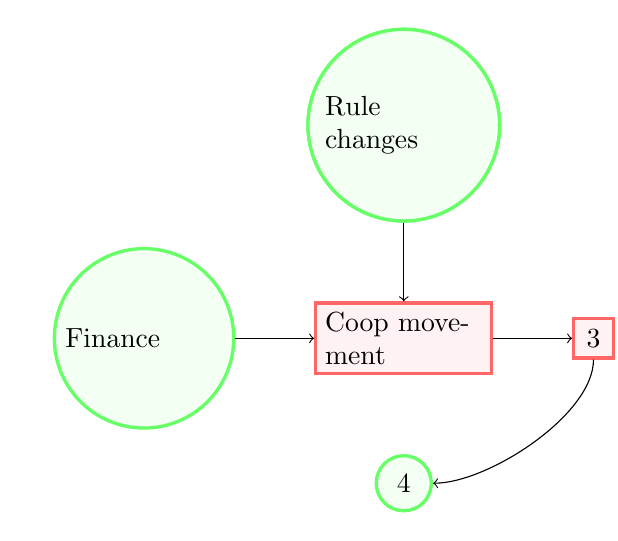
\begin{tikzpicture}[
roundnode/.style={circle, draw=green!60, fill=green!5, very thick, minimum size=7mm},
squarednode/.style={rectangle, draw=red!60, fill=red!5, very thick, minimum size=5mm},
]
%Nodes
\node[squarednode, text width= 2cm] (Coop)          {Coop movement};
\node[roundnode, text width= 2cm, text width= 2cm]  (uppercircle)       [above=of Coop] {Rule changes};
\node[roundnode, text width= 2cm, text width= 2cm]  (leftcircle)       [above=of Coop] {Rule changes};

\node[roundnode, text width= 2cm, text width= 2cm]  (leftcircle)       [left=of Coop] {Finance};

\node[squarednode]      (rightsquare)       [right=of Coop] {3};
\node[roundnode]        (lowercircle)       [below=of Coop] {4};

%Lines
\draw[->] (uppercircle.south) -- (Coop.north);

\draw[->] (leftcircle.east) -- (Coop.west);

\draw[->] (Coop.east) -- (rightsquare.west);
\draw[->] (rightsquare.south) .. controls +(down:7mm) and +(right:7mm) .. (lowercircle.east);
\end{tikzpicture}
\chapter{Lifeboat Canada}

\epigraph{ Canada must develop a humane housing strategy that supports rapid population growth, social integration and economic productiveness.  This is clearly a large-scale system design problem.}

\section{External forces}
Canada's current housing crisis and the projections of the previous chapter are mild compared to what we may face as the globe warms. Canada has committed to admitting  1.3 million immigrants over three years.   %Meanwhile housing  affordability has been declining since 2003-4, especially in Ontario, Alberta and BC.
If external world conditions remain as they are, the number of immigrants is likely to rise through the coming century. An annual increase of just  1\% each year (slightly less than the  rate of population growth for the last 50 years)  will raise immigration to nearly one million per year by the end of the century. The current growth is equivalent to adding one to four medium sized cities per year. That number will rise to as many as nine medium sized cities or one large city per year at the end of the century.   

External world conditions will not remain as they are, however.  According to a \href{https://www.pnas.org/doi/10.1073/pnas.1910114117}{study in the journal Proceedings of the National Academy of Sciences}\footnote{Future of the human climate niche, Chi Xu, Timothy A. Kohler, Timothy M. Lenton  Jens-Christian Svenning, and Marten Scheffer, May 4, 2020, 117 (21) 11350-11355.  %https://doi.org/10.1073/pnas.1910114117
}, the planet could see a greater temperature increase in the next 50 years than it did in the last 6,000 years combined. By 2070, the kind of extremely hot zones, like in the Sahara, that now cover less than 1 percent of the earth’s land surface could cover nearly a fifth of the land, potentially placing one of every three people alive outside the climate niche where humans have thrived for thousands of years. The result will be large scale migrations to the shrinking band of habitable lands.% A change in the geographical distribution of human populations  is  likely part of the spontaneous or managed adaptive response of humanity to a changing climate

Temperature will not be the only source of migration pressure. Kulp1 and Strauss\footnote{Kulp, S.A., Strauss, B.H. New elevation data triple estimates of global vulnerability to sea-level rise and coastal flooding. Nat Commun 10, 4844 (2019). %https://doi.org/10.1038/s41467-019-12808-z
} show – employing NASA’s nes Digital Elevation Model, CoastalDEM, that 190 M people (150–250 M, 90\% CI) currently occupy global land below projected high tide lines for 2100 under low carbon emissions, up from 110 M today. Under high emissions, CoastalDEM indicates up to 630 M people live on land below projected annual flood levels for 2100, and up to 340 M for mid-century.

Extreme weather events and conflict are the top two drivers of forced displacement in the short run globally. Since 2008, according to the United Nations High Commissioner for Refugees (UNHCR), an annual average of 21.5 million people have been forcibly displaced by weather-related events – such as floods, storms, wildfires and extreme temperatures.\footnote{
%https://www.unhcr.org/uk/news/latest/2016/11/581f52dc4/frequently-asked-questions-climate-change-disaster-displacement.html.  
See also Gaudry Haynie, J., Balagna, J., clark-Ginsberg, A. (2021) “Climate Change Migration: Developing a Security Strategy for All,” (https://www.rand.org/blog/2021/03/climate-change-migration-developing-a-security-strategy.html) who give suggest that nearly 30 million people  are displaced by weather and  conflict each year. Cited in the White House REPORT ON THE IMPACT OF CLIMATE CHANGE ON MIGRATION, October 2021. } The Institute for Economics \& Peace (IEP)  predicts that 1.2 billion people could be displaced globally by 2050 due to climate change and natural disasters.\footnote{
%https://www.prnewswire.com/ae/news-releases/iep-over-one-billion-people-at-threat-of-being-displaced-by-2050-due-to-environmental-change-conflict-and-civil-unrest-301125350.html
}. It is difficult to find anyone willing to make forecasts for the rest of the 21st century.\footnote{Projections assume that there will not be a mass die-off in this century as forecast by the 12972 Club of Rome Report, Limits to Growth", if society continued, as it has, on the ``Business as Usual'' path. }  



Canada, with its huge land-mass, relatively mild climate, stable government, high standard of living, and extensive agricultural capacity will be a preferred destination for many migrants. With perhaps one quarter of the most attractive land on earth at the end of the century, Canada is likely to receive or to be under  pressure to receive, a disproportionate share of global cross-border migration. It is unclear how many of those affected will look to Canada. An article in the UN Chronicle argues that, for several reasons,  it is ``improbable that there would be long-distance mass population movements even in a situation of systemic climate change.''\footnote{
%https://www.un.org/en/chronicle/article/will-there-be-climate-migrants-en-masse
}  Displaced people tend to stay near their origins, refugee camps and shelter villages are typically set up not far from the site of the calamity, countries resist cross-border migration, and various forms of adaptation are possible.  

Nonetheless, there is little doubt that Canada will have the opportunity as well as pressure to settle significantly larger numbers that currently envisioned. 
The country will face \textbf{the classic lifeboat problem}  described by by Garrett Hardin:\footnote{\textbf Garrett Hardin, BioScience Vol. 24, No. 10 (Oct., 1974), pp. 561-568 } how many are allowed aboard the lifeboat?  How many can the lifeboat sustain? how many will be left to die?

Faced with this dilemma, Canada can treat the situation as an opportunity to draw in far more talented and productive immigrants  than currently planned. 
 %Furthermore,  humanitarian considerations provide another motive for accepting far larger numbers of migrants.
The carrying capacity of \textbf{Lifeboat Canada}, however, depends on actions taken now - Will Canada have the capacity to house larger number of  immigrants given its difficulty in housing its current population?  Will Canada be able to integrate larger numbers into its economy? Will the country be prepared to quickly mobilize  the creative power of immigrants.

\section{The design challenge}
To prepare \textbf{Lifeboat Canada} for the opportunity and 
potential threat of mass migration and greatly increased immigration, Canada must develop a housing strategy that supports rapid population growth, social integration and economic productiveness. The strategy must be humane and environmentally sound. It has to draw on the pre-existing capacities of immigrants. This is clearly a large-scale system design problem.

\subsection{Features of the required system}

\begin{enumerate}
    \item High-density housing.
    \item Urban access
    \item High quality accommodation for families, including extended families  
    \item Environmental sustainability.
    \item Environmental quality for residents.
    \item Maintenance of the immigrant community structures and support for cultural continuity. 
    (Historically, much of the support received by immigrants has come comes from previously settle migrants.) 
    \item Connection to the resident community
    \item Supportive of commercial activities that generate income 
    and contact with others to accelerate economic integration.
\end{enumerate}



\documentclass[preview, 12pt]{standalone}
\usepackage{geometry}                % See geometry.pdf to learn the layout options. There are lots.
\geometry{letterpaper}                   % ... or a4paper or a5paper or ... 
%\geometry{landscape}                % Activate for for rotated page geometry
%\usepackage[parfill]{parskip}    % Activate to begin paragraphs with an empty line rather than an indent
\usepackage{tikz, pgf}
\usetikzlibrary{shadings, shadows, shapes, arrows, calc, positioning, shapes.geometric, decorations.markings,math,arrows.meta}
\usepackage{pgfplots}
	\pgfplotsset{width=7cm,compat=1.8}
	 \usepackage{calc}
\usepackage{mathtools,amssymb}
\usepackage{graphicx}
\usepackage{xcolor, colortbl}  
\usepackage{amssymb, amsmath}
\usepackage{epstopdf}
\DeclareGraphicsRule{.tif}{png}{.png}{`convert #1 `dirname #1`/`basename #1 .tif`.png}

\begin{document}
%%%%%%%%%%%%%%%%%%%%%%%%%%%%%%%
\section{Utility Function and budget}

\[ U=(G^\delta H^\beta  A_1^{\alpha_1}  A_2^{\alpha_2}A_3^{\alpha_31}\]
\[ U=(\frac{D}{p})^\delta H^\beta  A_1^{\alpha_1}  A_2^{\alpha_2}A_3^{\alpha_31}\]

\[pG=D=Y-M-\sum_jT_j\]

\begin{description}
\item[G]Hicksian composite good  (food) (for necessities $g$, use $G-g$)
\item[p]price index
\item[H]Housing  (for necessities $h$, use $H-h$. For houses sharing $H-s$ (for suite))

Housing can be a composite of size and other attributes: $H=H_s^(\eta_s) H_q^(\eta_q)\dots H_k^(\eta_k)$
\item[M] mortgage and housing costs 
\item[$A_i$] Amentity $i$
\item[$T_j$]Transportation cost $j$


\end{description}

\section{A Possible Typology of Models and Experiments}
While there  are very many variations on the basic urban model and many potential experiments with each model there are only a few of immediate interest if the goal is to text the ``resilience'' of equilibria.

These models may exhibit irreversibilities in variables such as distribution, homelessness, city form, and class structure. 


The  basic strategy for examining the system resilience is to shock a model (experiment) and then see if diagnostic variables recover. (This needs more precise expression.)


The first task is to select a subset of models an experiments that are of particular interests with respect to .

The second is to construct  a model that allows those case to be examined. Ideally the model would be easily adapted to other experiments.

The following is a an attempt to develop a typology with a clear  progresssive structure.

Feedback - wealth  allows  upgrading. This advantages the rich. Maybe this 


\subsection{Models}
\begin{enumerate}
\item \textbf{A: The Basic Model}

The workhorse of urban economics is the circular city model. Some feature of the central place generates rents. It may be that it is the only employment centre. It may be economies of scale to a single activity or synergies arising from various externalities\footnote{We are interested in agglomeration economies. The wage  structure would then be related to the population or industry  structure. Externalities driving agglomeration may be classified  into two types, the  or so-called ``Marshalian''  and ``Jacobs'' externalities.}. 


In the simplest model, the central place pays a uniform wage, $w$ to all employees, who have identical preferences and transportation costs. $w$ is an attribute of individual residents. Residents  purchase or rent equal quantities of land at differing locations $l$ for identical housing.  

There are transportation costs $T$ that depend on distance from the  central place, so land close to the central place is more attractive than land farther from the central place.  

The equilibrium concept is that a market with identical individuals with identical incomes and transportation costs will result in identical utilities. The result is that land rent must decline with distance from the central place to offset rising transportation cost. 

The size of the city is determined by population and lot size. Income and transportation costs will interact with lot size. The basic model can be initialized by matching the number of properties to the size of the population. 

If population exceeds the number of properties there are three margins to consider
	\begin{enumerate}
		\item The land supply can increase. There may be a conversion cost
		\item The land per-capita may decrease. This is not simple in a city with land-use regulations, zoning, and fixed capital in homes. A conversion process has to be defined
		\item A homeless population can emerge. 
	\end{enumerate}
	


It is convenient in this model to use a Cobb-Douglas utility function that has the property that a fixed fraction of income is spent on housing.  We can start with the assumption that earnings are fixed for the lifetime at the one-period wage, $w$. Then total spending on housing is $\beta Y, \beta <1$ and $ Y=w$. Let the transportation cost for a specific location $l$ be $T(l)$. The  equilibrium price at that location will be $P(l)= \beta Y-T(l)$.


It is convenient but not necessary to assume that land outside of the residential limit is costless. It is common to assume a fixed price for agricultural land. 

There is no fixed boundary and the size of the city is determined by the utility that can be achieved in competing regions of competing


\item \textbf{Y: The Basic Model with Income Differences}
This will result in segregation by neighbourhood depending on income. 

Income can be purely earning, which requires a distribution of $w$ across agents. Income  might include investment income, which  a private rate of return and a distribution of assets across agents. \footnote{A more subtle model could allow individual wages to be linked to the agglomeration of other workers - say engineers. we can imagine a city that has centres of agglomeration by profession or by complementarity. Depending on the production function, this should emerge endogenously.}
\footnote{Sufficient investment income could lead individuals to locate in cheap properties at the edge of the city.  Income might also be invested in property affecting the quality of a unit. This would require incorporating unit quality in the attribute list for each property, and introducing a quality preference  in the attribute s of residents.}


\item \textbf{L: The Basic Model with Locational Preferences}
This will result in segregation by neighbourhood depending on preferences.

One version would be include distance to the edge of the city as an amenity in the utility function. Another would be to locate amenities within the city. These would lead to higher prices near amenities.

A natural variant would be to have earning depend on location. If there were several locations  a polycentric city would emerge.

\item \textbf{T: The Basic Model with Varied Transportation Cost }
This will result in segregation by neighbourhood depending on income and Transportation costs. Experiments include cars for the rich and  transit. 

Diagnostics include change in total transportation cost and differential welfare effects.


\item \textbf{R: The Basic Model with a Rent-own choice}
This may result in the emergence of classes. Agents must have the capacity to borrow to purchase. Attributes of the agents and must now include  net assets,  an available interest rate, and a permissible mortgage.

We imagine a banker setting the mortgage rates and size. This can be done at the beginning of each period for each agent. 

With no income differentia we expect equal utiliites

\item \textbf{YR: The Basic Model with Earnings (Y) Differences and a rent-own choice}
This model is very likely to generate diverging classes as income differentials permit some to capture land rents from others. This is highly likely if borrowing costs decline with income and asset ownership.

\item \textbf{L: The Basic Model with Variable lot size}
This is achieved by making lot size a choice variable for households, in which case we will get a tradeoff between transportation cost and lot size and distance. Results for this model are known. Density  falls with distance from the centre. 

\item \textbf{YL: The Basic Model with Earnings (Y) Differences and Variable lot size}
The wealthy choose larger homes and lots farther form the centre

\item \textbf{S: The Basic Model with constant lot size and variable density}
This is achieved by allowing stacking of housing units. Results for this model are not known. This introduces a step change in housing form, and emphasizes unit size.

This model should produce some interesting spatial patterns, especially if couples with the possibillity of secondary central places.

\item \textbf{YS: The Basic Model with Earnings (Y) Differences, constant lot size and variable density}

This model should produce some interesting spatial patterns, especially if couples with the possibillity of secondary central places.


\item \textbf{IR: The Basic Model with outside investors and rent-own}

\item \textbf{IYR: The Basic Model with outside investors, Earnings differentials and Rent-own choice} This model is of interest if borrowing costs decline with income and asset ownership.



\end{enumerate}
\subsection{Experiments}
There are various experiments of interest. You will have to pick key ones. It is not necessary to do all of them in every model. 

	\begin{enumerate}
		\item increase population
		\item increase wage\
		\item add hard boundary (limit land)
		\item Introduce differential incomes
		\item Introduce differential access to capital
	\end{enumerate}

\newcommand{\cred}{\cellcolor{red!30}}
\begin{table}[htp]
\caption{Potential experiments: \textbf{Pick some}}
\begin{center}
\begin{tabular}{|c|c|c|c|c|c|}\hline

  &\multicolumn{5}{c|} {experiments}\\ \cline{2-6}
Model  &1 &2  & 4 &4  & \\ \hline
 A& \cred& \cred  &  \cred & \cred  & \cred  \\
 Y& \cred   & \cred   & \cred   &\cred    &\cred   \\
 T & \cred   & \cred   & \cred   &\cred    &\cred   \\
 R & etc &  &  &  & \\
 L &  &  &  &  & \\
 S&  &  &  &  & \\
 I &  &  &  &  & \\
 YR &  &  &  &  & \\
 IR &  &  &  &  & \\
  IYR&  &  &  &  & \\\hline
\end{tabular}
\end{center}
\label{default}
\end{table}%

\end{document}



\chapter{Background Rough Notes - Rent History Etc}

\section{Agglomeration discussion}

The phenomenon of growing productivity was initially identified and estimated in the economics literature production at the national level. The estimated functions linked capital and labour inputs to output.  Soon after the  earliest econometric models of output  were estimated, it was found that equations were not stable over time. Productivity grew over time
(We can do the arithmetic with the cobb douglas to illustrate) 

Faced with this puzzle, Robert Solow introduced a term that was time dependent, and an entire literature developed to explain this term. One productive stream explained growing productivity in terms of agglomeration effects- more people, more workers more firm or more diversity of firms appeared to be associated with growing productivity. Two major schools emerge - roughly speaking,  the Marshallian explanation, which emphasized firm-level processes and the Jacobs model which focuses on the creative effect of agglomerations of people in cities. Both have receives empirical support.

(We can do the arithmetic with the Cobb Douglas to illustrate)

Louis M. A Bettancourt and others applied similar models at the level of cities, but rather than a time-dependent term, they introduced a population-dependent term and found evidence from cities around the world that productivity rose as population rose: The scale of the city has a positive effect. The result  was one of a wide range of scaling results identifies in a great variety of systems examined in the complexity literature 


\section{Background}

\subsection{Inequality}
this wasn't how capitalism was supposed to work
wages part, 
over 50 for rent

\subsection{Drivers of the housing crisis}
supply and demand, stagnant income, and finacialization of housing

Several explanations of the current situation are commonly proposed. The first is simply that the problem of housing is a supply and demand problem where supply is blocked by some features of urban regulation. The second explanation is that the distribution of income has changed in some way that mean a significant fraction of the population are unable to afford satisfactory housing, and therefore this is the problem that must be solved.  The third common explanation currently is that financialization of the housing market  is changing the way the city economy is working, redistributing income and potentially threatening the long term growth and wealth creating capacity of the city.


\subsection{How we do the resilience analysis}

- what will we do? *** 



\section{Rent, Production and the City: Who Gets the Wealth}


%The sources of economic growth and the distribution of income are themes that run through the history of economic thought. 

The story of rent is the story of 

two great theories of distribution
a methodological evolution from descriiption to calculus to complex systems and an evolution of the economy 
from agriculture to indsutrial produciton, to social scaling or wealht in cities. 



There are two great stories of distribution in economics. The first and oldest is rent, %the classical work on rent, going back to 
developed in Ricardo, in which owners of an asset are able to extract a value beyond what they contribute. 
The second is the marginalist approach, developed by Clark and others, looking at a scenario in which workers receive the marginal value of their contribution to production. This tradition dominate in neo-classical economics, particularly in the United States, and %formed the basis of conventional micro-economics training.
% it gave a story of production that seemed to align with the rising fortunes of ordinary people/workers following WWII, in the 1950s and 1960s when it came to dominate. 
% formed an intelectual foundation for anti-monopoly political movements in the early 20th century. 
This work contributes to a third theory of 

emergent complex systems methodology and  work on urban science, the power law concentration, and integrates/ to achieve a sysnthesis of  the clasical descriptive work on rent and the neoclassical marginalist appraoch

These stories are, at their heart, stories of who claims what share of production. They evolved within an evolving theory of production. The early stories of production thinkers like Ricardo focuses on were agricultural. Who claimed the surplus from agricultural production? Over time, the story moved to industrial production, and increasingly urban- with the social wealth of cities/human capacities developed in cities dominating. % Later thinkers including Smith and Marx%leaving aside purely inherited weath- as that becaumse caught in this same circuit of capital transforming from production, to money and back. 



Methodological-- early discririptive theories told rich layered stories with different
The excitiment concentrated  calculus.. in the classical distributional dynamic.

The complexity - allows for tracing the paths of individual- what happens for whom under a far broader range of conditions

The clarity of pedagogical methcs- bottom up and top up both have illustrative cases e.g. edgeworth box or the schellings/birds models.
But true theory integrates in something that moves between scales fluidly, makes itpossible for the distinct scale based approaches to come together.


Complexity

Early discriptive work
This explosion of formal rigour - focused attention.. 


And the political context..

Monopoly- political pressure real explosion ofwealth creation-- economic success of political efforts to break up monopolies.
And a dynamic- lots of worker power- expanded equality-- workers seemed strong, 
As well as the political environment in the US during the cold war, older stories rooted- marx- repression, ednomists perhaps created an envronment in which economists
a side fo the economcs

-- methological pdrived moved the point whre discriptive and historical appraoches baredly taguth.

Samuelson-- successful exciting-- formal-
a generation
created micro, macro
-- at the moment of the baby boom- departments founded in this moment of exuberance. raised in it, taught according to this framework.


Computers took over from calculus -Brian Arthur
Cities took over from industries - concentrated value-- finance- and law main power centers.. - eigen value centrality.

Crisis in 2008 -- reintroduced dscrptive
Methodologial
Cities-- power law dist. rising debt and inequality. -- unstable and financialize.d
Increasing inequality, risind debt. - worker power expanding wages and equality, a story that explained- vs subsistence.


Exactly what those pattnersnew methods are so succesful are what was lef tout..



Polarized in the periodo of the cold war - the discussion of the market-- perhaps a tendency to avoid the distributionl.. Revolution and drama.



Early theories were implicit. They have the same logic- but exist in words

mathematization was important to the simple centrality of marginalism.






With Clark
A second great theory of distribution
The result is much of the theory of rent was lost. 
time

While Marx emphasized the tendency towards consolidation and exploitation in markets, Clark saw the tendancy to increased competition. 

This allocation— dynamic quality of how wages evolved
They are bidding- and it will converge 
What share do workers get- subsistence wages- get 
But as output grows, and as firms compete for labour, particularly skilled labour, is that a sufficient experience.



Three drivers
Calculus had limits.
The political moment of expanding wages with a labour sector in a position to negotiate as the economy rebuilt following WWII and destruction of old wealth— dynamic time. 
Following WWII with growing demand for labour labour could bargain, 
Following WWII in the period— subsistence waves tending— when labour could bargain,
Following break up some of the largest monopolies like in steak— general steal


Also coincided with the political movement McCarthiesm perhaps led scholars to de-emphasize the connections of their work with the classical socialist litturatue.
Mathematical economics became an exciting and dynamic area.

Until this point the theory was largely descriptive..
xx Cobb working with Douglass developed a formulation — exponential, in economics their names have remained associated with the xyz formulation. 

Clark made a case it was just- became problematic.
Doesn't actually happen -- and not jsut

OUR CASE IS THAT IT FALLS OFF A TOTALY DIFFERENT CLIFF



Economics had theories with rich dynamics, concerned 
Classical economics was concerted with ownership and wealth. But they were largely descriptive.
But the new calculus struggled to deal with stocks and with dynamics. 
(Came back with forester and other systems theory, as well as complexity etc.)

The French Engineers in the school of bridge end road used calculus early .. followed by xyz
Technical development and intelleual excitement aligned
Became very exciting dynamic, had many success - took over the discipline. 
Tied with political successes breaking up big monopolies — seemed to offer a path forward

US opposed soviet ideas and an intellectual environment that may have led academics to dephasize the aspects of their thinking connected with classical socialists thought. 

In this environment a particular approach became dominat— also at a moment when schools and departments were growing— the baby boom came to universities at the moment of Samuelson’s peace micro-macro divide gave a tool kit to a whole generation of economists— 

Embedded at the heart of micro- the satisfyingly precise formal structure of calculus.. the marginalize appraoche— 
Thus came to define a new disciplien— a formalization of Econ.. 
Extensions from that base became the defining advances of a generation of American economists..
Attracted math- a feedback loop.

Less emphasis on intellectual history, how changing- heterodox.. all the full range of thought

Including the much more exiting new techniques of complexity and systems- opening in 2007 an explosion of these techniques in the economies. 




CITIES

But cities matter more and more
Jacobs theory of wealth and value as fundamentally social.. 
Combined with xysz. Jacobs did

Now complexity and scaling theory revealing the universality of those principles advanced by Jacobs..

This requires a different formulation of rent… - and production wealth is inherently social what are the implicaitons— what does that mean.. 






In our model, land comes in implicitly through the demand for labour. 


\section{Chapter: Draft Literature Review and Background}

\section{Background}
\label{Sec:Background}
\newpage
Our approach/model is constructed, drawing together pieces from a number of research areas from economics and the study of cities, including rent theory, production functions, the standard urban model, growth theory, urban growth theories, financialization and the theory of distribution. 
We relate this to the scaling models from the study of complexity. This gives a deeper look at distribution in the cities, the effect of financialization, and effect of both of these on the growth and development of cities. 

The literature makes it clear that the cost of transportation is crucial, the cost of housing is crucial, and that there are strong pervasive agglomeration effects driving productivity and population growth. (City population is observed to follow a power law distribution.)

We are interested in agglomeration economies. The wage  structure would then be related to the population or industry  structure. Externalities driving agglomeration may be classified  into two types, the  or so-called ``Marshalian''  and ``Jacobs'' externalities


3 lines  
- production leading to Jane Jacobs
- cities leading to Jane Jacobs
- scaling factors and complexity leading to Jane Jacobs and empirics in a theory of cities

2 theories of production

Ricardo
Ricardo’s rent theory explained class and the distribution of income in terms of the the productivity and ownership of land in an agricultural society. Land was the scarce factor in production and control of land allowed landowners to extract any production in excess of the agricultural wage. Ricardo could assume that labour was in surplus and therefore the agricultural wage would approximate the subsistence wage. 

Marx
Marx adapted the Ricardian model to an industrial society in which surplus product could be used to create more capital and largely ignored land rents. He retained the subsistence wage, and explored the effect of reproducible capital.

Clark
Clark %\footnote{and Wicksteed} extended the theory of rents to produce 
elaborated a neoclassical distribution theory that tied income to the marginal product of each factor for a firm in a competitive economy rather than class ownership of capital. 
This marginal productivity theory became dominant SOME BENEFITS.. Although the marginal productivity theory became dominant in economic thinking, rent theory retained an important explanatory role in resource, agricultural, regional and later urban economics and even sports economics. 

Clark %\footnote{and Wicksteed} %extended the theory of rents to produce 
elaborated a neoclassical distribution theory that tied income to the marginal product of each factor for a firm in a competitive economy rather than class ownership of capital. Although the marginal productivity theory became dominant in economic thinking, rent theory retained an important explanatory role in resource, agricultural, regional and later urban economics and even sports economics. 

Rent theories have remained at the centre of economics despite the development by Clark (1894) of the more modern theory of distribution in which factors ideally receive the value of their marginal product. In modern welfare economics a measure of surplus that is the direct descendent of Ricardian land rent is at the core of the First Theorem of Welfare Economics, arguably the most significant theorem in the social sciences. With Alonso (1964), another another application of rent theory became the foundation of modern urban economics.

\section{Exploitation}
John Roemer’s 1982 Class Exploitation Correspondence Principle (CECP) states that producers who optimize by only selling labour are exploited at the economy’s equilibrium, and agents who optimize by hiring labour are exploiters. Exploitation and class structure are shown to arise from differential endowments in a manner consistent with both Ricardian explanation of class incomes and Marx’s conception of exploitation. We extend the argument to show that differential access to finance capital, urbanization, the growing importance of human capital in producing surplus and agglomeration economies endogenously generate a class structure based on the indirect capture of land rents, We illustrate the emergence of class structure within a simple agent-based model of the land market in a monocentric city. The model is consistent with the theories of Ricardo and Henry George in locating the ground of exploitation and class in the capacity to extract social surplus through land ownership, and differs from the standard Marxian analysis in its reliance on access to financial capital rather than control of productive physical capital.

The sources of economic growth and the distribution of income are themes that run through the history of economic thought. 

From Smith and Ricardo economist have understood that the net product of the economy is divided among functional classes.
 Ricardo is generally credited with providing the best early description for the division of the product of the land between labour and property owners. 
 Marx is generally credited with providing a convincing explanation based essentially on Ricardo's insights, of the distribution of the product of industrial capital with a class-monopoly on ownership the capital,  as well as insights about the evolution of a society based increasingly on produced rather than natural capital. 
 Henry George elucidated the role of land rent, particularly in the urban context as as a mechanism for extracting socially produced economic surplus.  

The division of the product of the earth among the classes of society has been a central issue in economics since at least Ricardo presented his theory of  rent, through Marx, adapted the concept of rent to an industrial and capitalist economy and Henry George, who applied it in the urban context. Land rent is also at the core of modern urban models.  John %\textcite{RoemerGT} 
in \textit{A General Theory of Exploitation and Class} 

%\textcite{RoemerGT} 
%\footnote{\cite{RoemerGT} p12} 

The distribution of rent, where it goes, and what the implications are. 

\section{Liturature Review}

3 lines  
- production leading to Jane Jacobs
- cities leading to Jane Jacobs
- scaling factors and complexity leading to Jane Jacobs and empirics in a theory of cities

2 distributional stories.
- class and rent -- synthesis of rent and class--

Then is the history of rent seperate?

O’Sullivan (2011) identified “five axioms of urban economics” that have emerged from a century of study: (a) location-specific costs and benefits balance to generate a locational equilibrium; (b) self-reinforcing effects induce concentration of activities and individuals; (c) externalities are prevalent; (d) production is subject to economies of scale, which favours agglomeration; and (e) competition generates zero economic profit. These features combine to produce dynamic urban system that will shape our future. 

We build a model that incorporates the five “axioms” to demonstrate how production externalities, in a class of models, can drive urbanization, class formation and the wealth distribution.

To understand the relationship requires integrating the distributional appraoch from clasical economic theory of rent with the modern marginalist model of distribution through wages. It does this by integrating the urban model with the model of production and including the cost of land and transportation in the urban wage in the labour costs. 
In this way the two factor model of projection reflects the clasical landowning extraction of rents by landowners, with a model of wages in competitive markets. 

\subsection{Rent}

 What Is Economic Rent?






neoclassical story.
Economic rent is an amount of money earned that exceeds that which is economically or socially necessary. This can occur, for example, when a buyer working to attain a good or service that is considered exclusive makes an offer prior to hearing what a seller considers an acceptable price. Market imperfections thus lead to the rise of economic rent; it would not exist if markets were perfect, since competitive pressures would drive down prices. 
%https://www.investopedia.com/terms/e/economicrent.asp
% https://www.wallstreetmojo.com/economic-rent/



Henry George brought the classical position to its logical conclusion: rent is an unearned increment. The Classical Base of Modern Rent Theory, Conway L. Lackman
“Whatever part of the produce or… of its price, is over and above this shame” (which pays for the capital advanced “together with the ordinary profits”), “he” (the landlord) “naturally endeavours to reserve to himself as the rent of his land” ([O.U.P., Vol. I, p. 163; Garnier,]  
l.c., p. 300). Theories of Surplus Value, Marx 1861. [Chapter XIV]  
 Adam Smith’s Theory of Rent [1.  Contradictions in Smith’s Formulation of the Problem of Rent]
This excess may “he considered as the natural rent of land” ([O.U.P., Vol. I, p. 163; Garnier,]
l.c., p. 300).


 \subsection{Ricardo}
 
 David Ricardo developed a theory of land rent.
Leading figure in classical economics



He modelled the agricultural economy.
Ricardo developed the idea of 

He was friends with James Mill, Jeremy Bentham and Thomas Malthus.

He theoriezed the agricultural economy.





\section{Drafting REVIEW}
This section traces the history of rent and production in economics.
 central issue in economics since at least Ricardo presented his theory of  rent, through Marx, adapted the concept of rent to an industrial and capitalist economy and Henry George, who applied it in the urban context. Land rent is also at the core of modern urban models.  


In economics, rent is a surplus value, i.e. the difference between the price at which an output from a resource can be sold and its respective extraction and production costs, including normal return (DFID, 2003; Luchsinger \& M\:uller, 2003; Sharp, 2003; Stoneham et al., 2005).

Chapter 24: Doctrine of Adam Smith concerning the Rent of Land
``Such parts only of the produce of land,” says Adam Smith, ``can commonly be brought to market, of which the ordinary price is sufficient to replace the stock which must be employed in bringing them thither, together with its ordinary profits. If the ordinary price is more than this, the surplus part of it will naturally go to the rent of land.

If it is not more, though the commodity can be brought to market, it can afford no rent to the landlord. Whether the price is, or is not more, depends upon the demand.''

More briefly, rent is a surplus value after all costs and normal returns have been accounted for. Normal costs include  payment of all the factors of production at their market rate.(Labour at the going wage, Capital at the interest rate, supplies at their normal price). The great social question at first was who gets the surplus.  

%The question was pressing because it appeared that landlords were capturing the surplus without contributing to production while may peasants were very poor. 

Ricardo

% Born in the late 1700s, was a British poltical economist. The son of a stockbroker, he built a fortune by investing.
The law of rent was formulated by David Ricardo around 1809, and presented in its most developed form in his magnum opus, On the Principles of Political Economy and Taxation. This is the origin of the term Ricardian rent. Ricardo's formulation of the law was the first clear exposition of the source and magnitude of rent, and is among the most important and firmly established principles of economics.

The landlord would rent out all the land which generated at least enough to pay all the costs. Anything in excess of the costs could be charged as land rent to a tenant farmer.

This excess, or surplus, he identified as the income of the landlord. The landlord captures the surplus by ownership of the natural resource land. 

Ricardo, did not write down a production function his, but his analysis can be understood as implying one.

Clearly in his model there are two basic productive factors, land and labour. The landlord  receives the surplus generated by the land and the rest of the value of production goes to labour. Ricardo essentially assumes that there wage is  just sufficient to reproduce the labouring class.\footnote{``In the natural advance of society, the wages of labour will have a tendency to fall, as far as they are regulated by supply and demand; for the supply of labourers will continue to increase at the same rate, while the demand for them will increase at a slower rate.''  This is  basically Malthus.} He has explained the distribution of the fruits of the land among the main classes of the economy.

The implicit production function is
\[Y=F(N, L)\]

Where the output $Y$ is a function of $N$, the number of workers and $L$, land.

His analysis included a concept of diminishing marginal return, the rate at which production grows declines. 
This shows in his use of the terms ``extensive margin'' and ``intensive margin'' to explain the income of the landowner. He focused on the difference between the cost of production on a unit of land and the revenue generated. 



employers enjoy a bargaining advantage over workers and can coerce them to accept worse terms, because they need individual workers less than individual workers need employment. It is no surprise Marx was an admirer. Wages are not the simple product of supply and demand in Smith; bargaining asymmetries are key.

Ricardo included concept of diminishing marginal product, which means


His analysis can be understood in terms of a production function. 
% Factors of production are things that play a role in creating the output. There are several factors of production, things required for production/to create wealth/value (using capital and labour). Most obviously capital and labour. One of the factors of production is labour. In principle the rate at which hiring changes output can take any form. If hiring one more worker increases output, the marginal product of labour is positive. The marginal product can be positive and increasing, or positive and decreasing. If the marginal product of labour is decreasing, the curve is slopes downward, there are decreasing returns to scale, and each additional worker adds less to output than the last. % DIAGRAM  In general hiring more people increases production. In general employers choose workers who would increase production. Otherwise they would not hire. Returns to scale determins how much hiring one more worker increases output. With increasing returns to scale, each new worker increases output more than the last one did, and companies tend to grow big. With decreasing returns to scale, each new worker increases output by less than the last one did and so more, smaller companies may form % (TODO: clarify explanation of implications). To connect with the tradition of analytic economic modelling, ensure there is an equilibrium, by making the marginal product of labour monotonically declining, ors declining over the whole function. This equilibrium condition ensures the curve in the diagram is slopped downward and the curves intersect. % (TODO: discuss/justify assumption, ground empirically)


 2 factors is typical since it's enough for most kinds of analysis. Another factor typically used to introduce another constraint on production, or potentially consumption. Eg. labour is mobile, capital takes time to accumulate but you can put it anywhere, but forest is a flow from the ground-- puts a limit on the region of the city. - land, flow from the land, natural resources.
 
 The factors are usually chosen so xyz
 To keep it tractable- one which is slow to adjust and one which we can adjust quickly - one which is world/embodied work and one which is current work, the rest falls between.

%and is replaced with capital. -- What you'd do an analysis if you put in 30 factors, in the analysis you hold 28 and let 2 move to see what's going on, and what you get is - you have a production function with certain mathematical factors, you can expand as much as you want. you can expand as much as you like-- everything you deduce about 1 is true about any 1 and all the rest if they hold the same functional relation to one another.This is a mathematical trick that gives you xyz.. things you get from it are things like there's a good reason to assume growth till you get 0 profit, then you get competitive markets, all that drops out of the math. - profit maximization you can impose, expansion to 0 profit, expansion till marginal product of labour equals the wage, value of marginal product of capital equals the interest rate, marginal product of whatever is equal to the price/unit of whatever it is - 


Historic evolution is land and labour.

Marx


, as we move from agriculture, 





John Roemer’s 1982 Class Exploitation Correspondence Principle (CECP) states that producers who optimize by only selling labour are exploited at the economy’s equilibrium, and agents who optimize by hiring labour are exploiters.

Roemer
RoemerGT demonstrates that in equilibrium there are classes that are exploited and classes that are exploiters, as well as intermediate cases, using  a definition a definition of exploitation 

that is essentially Marxian and is consistent with Ricardo's rent theory and that of Henry George: 
%\begin{quotation}
%
An agent is exploited  if and only if the value of the labour the agent sells plus the value of own production plus wage earnings is less than the maximum value of their consumption bundle.
%\vspace{.25cm}
%
%and\vspace{.25cm}
%
%An agent is an exploiter  if and only if the value of the labour the agent sells plus the value of own production is less than the minimum value of their consumption bundle.
%\end{quotation}

A General Theory of Exploitation and Class examined a General equilibrium linear economy in which all individuals rationally choose their  activities given their initial endowments and demonstrated  the endogenous emergence of a class structure in a purely neoclassical model. 

Marx
distribution of the product of industrial capital with a class-monopoly on ownership the capital,  as well as insights about the evolution of a society based increasingly on produced rather than natural capital. 



CITY
Rent howerer has remained central in the study of the city
Began everywhere.

Johann Heinrich von Th\"unen was influential in developing the spatial analysis of rents, which highlighted the importance of centrality and transport. Simply put, it was density of population, increasing the profitability of commerce and providing for the division and specialization of labor, that commanded higher municipal rents. These high rents determined that land in a central city would not be allocated to farming but be allocated instead to more profitable residential or commercial uses. 


 Henry George elucidated the role of land rent, particularly in the urban context as as a mechanism for extracting socially produced economic surplus.  

OLD?
 
Ricardo developed a theory of land rent. He did not write down a production function, but he quite clearly understood and used the concept of diminishing marginal product. This shows in his use fo the terms ``extensive margin'' and ``intensive margin'' to explain the income of the landowner. He focussed on the difference between the cost of production on a unit of land and the revenue generated. The landlord would rent out all the land which generated at least enough to pay all the costs. Anything in excess of the costs could be charged as land rent to a tenant farmer.

This excess, or surplus, he identified as the income of the landlord. The landlord captures the surplus by ownership of the natural resource land. 

Clearly in his model there are two basic productive factors, land and labour. The landlord  receives the surplus generated by the land and the rest of the value of production goes to labour. Ricardo essentially assumes that there wage is  just sufficient to reproduce the labouring class.\footnote{ ``In the natural advance of society, the wages of labour will have a tendency to fall, as far as they are regulated by supply and demand; for the supply of labourers will continue to increase at the same rate, while the demand for them will increase at a slower rate.''  This is  basically Malthus.} He has explained the distribution of the fruits of the land among the main classes of the economy.

The implicit production function is

\[Y=F(N, L)\]

Where $N$ is the number of workerrs

\subsection{Marx}
 Marx examined a developing manufacturing economy. In this economy the owners contributed the machinery, buildings, and even working capita to fund the workers until the product can be sold. This contribution must be accumulated from their profits in the preceding cycle of production,  and has to be reinvested once the revenues of the current round have come in and the bills have been paid. Marx actually describes a circuit of capital from its for as money to its form as physical capital. 
 
 
The implicit production function is

\[Y=F(N, K)\]
where $K$ stands for the productive capital stock. 

As in Ricardo, labour is in surplus and capital is scarce. As in Ricardo the scarce factor owned by a special class - now the capitalists, is able to appropriate the is able to capture the surplus value. Like Ricardo,  marx saw the appropriation of surplus as without morel justification - 


Marx also pointed to a new dynamic in capitalist systems - that productive capital is not fixed as land is, but does and must expand as surplus is reinvested. The expansion will eventually outrun the expansion of demand and the rate of return will fall, leading capitalists unwilling to invest and creating a crisis,.


 
\subsection{Henry George} 
  Henry George returned to land rent with a new insight based on the emergence of the capitalist city. Since land rent is unearned income he argued that it should be seen a social income - that it could be used to pay for all the needs of the community. This is the basis of the `single tax' movement. He cleasrly looks back to Ricardo and the early rent theory, but also forward to urban models. His analysis would be recovered in urban models with the proof of. the `Henry George Theorem" in... by .... It demonstrated that if it was some ;public good that attracted people to a city, the optimal level of the good was jus the amount that could be paid for from the increment in land value.\footnote{Progress and Poverty: An Inquiry into the Cause of Industrial Depressions and of Increase of Want with Increase of Wealth: The Remedy is an 1879 book by social theorist and economist Henry George.}
  
  Wikipedia expresses the dynamics this way: ``The tendency of speculators to increase the price of land faster than wealth can be produced to pay has the result of lowering the amount of wealth left over for labor to claim in wages, and finally leads to the collapse of enterprises at the margin, with a ripple effect that becomes a serious business depression entailing widespread unemployment, foreclosures, etc. ''
  
  In George land includes all natural resources, everything ``that is freely supplied by nature.''  
  \footnote{Analysis of the locational rents generated in this class of models has resulted in several authors demonstrating the validity of variants of the Henry George Theorem (\cite{Arnott-Stiglitz79, Arnott04, BehrensKanemoto14, JohnM.Hartwick1980THGR}). These analyses  show that the land rents can exactly equal the cost of the public good that draws individuals to the city or the production services that draws firms. In our model these rents are extracted by land-owning financial capital. They are not invested in a public good or in expanded production capacity.}
  
  \subsection{John Bates Clark}
  Another socialist like George, he was also one of the pioneers of marginalism. By 1986 he was praising the dynamical process of competition partly in opposition to the single tax movement George had initiated.  His (1891). ``Distribution as Determined by a Law of Rent,'' argued that, given  competition and homogeneous factors of production labor and capital, the division of the social product will be according to the productivity of the last physical input of units of labor and capital.\footnote{Responding to the "indictment that hangs over society" that it involves "exploiting labor," Clark wrote:

    It is the purpose of this work (his 1899 'Distribution of Wealth) to show that the distribution of the income of society is controlled by a natural law, and that this law, if it worked without friction, would give to every agent of production the amount of wealth which that agent creates. However wages may be adjusted by bargains freely made between individual men (i.e., without labor unions and other "market imperfections"0, the rates of pay that result from such transactions tend, it is here claimed, to equal that part of the product of industry which is traceable to the labor itself; and however interest (i.e., profit) may be adjusted by similarly free bargaining, it naturally tends to equal the fractional product that is separately traceable to capital.} 
  
 \subsection{Cobb and Douglas}
 The neoclassical revolution opened the use of formal functional mathematics and calculus. Cobb and Douglas (notably Cobb) came up with a specific and very convenient functional form that captured much of what economists were talking about:
 
 \[Y=AK^\alpha L^\beta\]
 
 Where $A$ is a constant scale factor\footnote {apparently previously used by Knut Wicksell, Philip Wicksteed, and L\'eon Walras. I didn't know that!}. The Cobb–Douglas form was developed and tested against statistical evidence by Charles Cobb and Paul Douglas between 1927–1947. It was  the widely circulated empirical work seems to have permanently associated the rather familiar function with the two names for economists.
 
 A 2021 meta-analysis of 3186 estimates concludes that "the weight of evidence accumulated in the empirical literature emphatically rejects the Cobb-Douglas specification."\footnote{Gechert, Havranek, Irsova, Kolcunova (2021), "Measuring capital-labor substitution: The importance of method choices and publication bias", Review of Economic Dynamics, doi:10.1016/j.red.2021.05.003, S2CID 236400765}
 
 The form captured  important regularities in the data but these drifted over time. 
 
 %COBB DOUGLASS additive property-- multiplicative.. additive property-- expandibile in the sense you can add more in-- some functions which are copb douglas which is log linear so seperable, and so additive in an important sense. BUT MVP is true for any firm successfully multipled function even if pruduction function is not seperable..
 
% Write profit using input, profit, - differentiate, get first order conditions which are a peak in the profit function, take those and manipulate to get rules, features of the optimal behaviour-- set marginal value equal to the price, set quantity to the point where profit goes to zero.. approach to standard economics..
 
 \subsection{Solow}
To deal with the drift, Solow introduced a refinement, opening the field for a further series of refinements  in an enterprise that became known as ``growth theory.'' \footnote{A Contribution to the Theory of Economic Growth,  Robert M. Solow, The Quarterly Journal of Economics, Vol. 70, No. 1 (Feb., 1956), pp. 65-94. Stable URL: http://www.jstor.org/stable/1884513}

Solow argued ``As a result of exogenous population growth the labor force increases at a constant relative rate n,'' so
  \[L(t)= L_0e^{nt}\]


 \[Y=A(t)K^\alpha L^{1-\alpha}\]
 where $A$  explains the change in factor productivity as a function of time. It is no surprise that adding a variable allowed the model to track the data better. Solo went further, and described the dynamics of the model using an explicit time dependence: ``As a result of exogenous population growth the labor force increases at a constant relative rate n,'' so
  \[L(t)= L_0e^{nt}\]
  
  
 As a result, if we stick this into the production function 
 \begin{eqnarray}
 Y&=cK^\alpha (L_0e^{nt})^{1-\alpha}\\
    &=c(e^{nt})^{1-\alpha}K^\alpha L^{1-\alpha}\\
    &=A(t)K^\alpha L^{1-\alpha} \label{Eq:Solow}
 \end{eqnarray}
 where
 \[A(t)=c(e^{nt})^{1-\alpha}\]
 
 N. Gregory Mankiw, David Romer, and David Weil created a human capital augmented version of the Solow–Swan model that can explain the failure of international investment to flow to poor countries.

    \[Y(t)=(A(t)K(t)^\alpha H(t)^\beta L(t))^{1-\alpha -\beta} \]
    
    From the Solow example, we can see that if all the time functions are exponential we end up with equation~\ref{Eq:Solow} again.
    
\subsection{How the Solow model performed}    
The estimated model explained 78\% of variation in income across countries, the estimates of $\beta$ implied that \textbf{ human capital's external effects on national income are greater than its direct effect on workers' salaries.}%(\url{https://en.wikipedia.org/wiki/Solow\%E2\%80\%93Swan_model)}.  
    
Theodore Breton provided an insight that reconciled the large effect of human capital from schooling in the Mankiw, Romer, Weil model with the smaller effect of schooling on workers' salaries. He demonstrated that the mathematical properties of the model include significant external effects between the factors of production because human capital and physical capital are multiplicative factors of production.[20] The external effect of human capital on the productivity of physical capital is evident in the marginal product of physical capital:

    \[ MPK={\frac {\partial Y}{\partial K}}=\frac {\alpha A^{1-\alpha }(H/L)^{\beta }}{(K/L)^{1-\alpha} }\]
 
 \subsection{Endogenous growth theories}  
 Endogenous growth theories make the increase in factor productivity depend on  optimizing decisions about human capital investment, invention, and investment in technology improvement.  
 
  Productivity growth results from an active search process for innovations in
which the ability to appropriate profits determines the resources devoted to
innovative activity (OECD, 1992, Crafts, 1996). Growth depends on the incentives to in-
vest in improving technology.% https://link.springer.com/chapter/10.1007%2F978-1-349-26732-3_13
 
  I don't think these models are much help in understanding cities, which appear to become more productive and population rises. this is an agglomeration effect.



\subsection{Solow MORE K}

The firm maximizes profit by setting the marginal value of the product of each factor equal to the unit cost per factor. 

This ensures that the marginal rate of technical transformation equals the price ratio. 

*** WHAT IS THE PRICE RATIO

the marginal rate of technical transformation is the (neg) slope of the indifference curve, 
- technical since it's a technology, the production function represents a technology, and you have inputs-- you can maintain one output by substutiting one input for another, you can see them as transfromation (substitution)
- changing technology changes the shape of the curve.. ---note growth theories takes technology out of the term-- growth is a term up front.. on avg it's bringing the whole thing up. consistent with the scaling term-- there is this pre-factor that changes a lot- e.g. china to US-- 

NOTE AALSO  the pre factor is by nation not just time-- policy matters weath matters, geopolitical context matters.. a. lot. - US is 8x larger than china 27x larger than nigeria (CHECK NUMBERS..) .. bus driver paid x less.


the indifference curve is the curve along which output stays the same as you supstitute labour for capital or vice versa. 
the optimum input mix, it turns out, is where the isoquant (equal quantity - indifference to quantities curve vs indifference to utilities curve) of the production fuction equals output line is tangent to a cost constraint..

curve tangent to a straight line at the optimum-- at the straight line is the price  ratio

the wage over the interest rate. 

ALTERNATIVE FUNCTIONAL FORMS FOR UTILITY FUNCTIONS AND PRODUCTION FUNCTIONS
isoquant measure how things you eat make you happy-- the production function that has that isoquant is measuring equal outputs
vs indifference curve. .. that has the utility-- is measuring happiness, but they are both the same kind of geometric mean of the inputs. 

Examples whrere the isoquant would not euqal the indifference curve include: -- leiontief for instance- right angle corners with 0 substitution . 2 shoes in a pair. need a left and a right one, two right one doesn't help at all. in that case they're perfect complents not subsitutes
if they're straight line, you have perfect substittes a.. 




\subsection{COBB DOUGLASS PROPERTIES}

We use a Cobb Douglass function for production because it has convenient properties -- you can control the degree of degree to return to scale simply by varying alpha and beta. secondly alpha turns out to be under the marginal productivity interpretation of income and optomixation, it ends up being the share of income that goes to capital and to labour- ends up being the elasticity of capital with respect to labour or elasticity of capital with respect to labour.. very much a funcitonal form in line with the scaling  appraoch and they come to the same.. -let's you talk about your returns to scale naturally and ascribe them as you will. it also -- really convenient form used throughout econ for illustration, it has been estimated, and it can be derived alternatively as the form you can look for from the scaling research..]
*** XYZ properties,

cobb douglass has another trait, which is it's a constant elasticity of substitution fuction.
elasticity of subsstittuion combines the slope and the amt of inputs. . easy to slow graphically CEF - constant elasticity of substitution.




Growth theories have several components
the amt of each you have

e.g. if an economy increases the labour or capital it has, it can move to a higher isoquant. if it increases 1 it can move to a higher isoquant-- that doesn't change the shape-- you can move since you have more inputs.

if you have technical change that makes 1 factor more productive.. imagine a nice smooth isoquant.. and it takes some labour that puts you on that isoquant.. if the labour got more producteive, the same amt of labour would move you to a higher isoquant.. cou..


Solow swan puts tech to the front-- the prefactor containts tech growth

we actually put the factor of production into the prefactor.. ** 



% Note on functional form: The analytical approach looks at marginal product and curvature of these functions -- so all we need is something with a curvature and a marginal product in each factor that you put in -time capital, labour 1, labour 2, labour 3.. our focus is on the local curvature and the slope.
%(\cite{Solow56, Swan}), 


VARIATIONS

There are all kinds of other things that could be included in Solow-Swann. For instance, the Mankiw–Romer–Weil version of the model adds a term for human capital.

The general form can be extended in many ways 0 
 In principle it could be restrictred offer time, different workers, firms, sectors, neighbourhooods, evolving over time.


\subsection{Exploitation}\label{Sec:Exploitation: A Note}
The division of the product of the earth among the classes of society has been a central issue in economics since at least Ricardo presented his theory of  rent, through Marx, adapted the concept of rent to an industrial and capitalist economy and Henry George, who applied it in the urban context. Land rent is also at the core of modern urban models. 
%John \textcite{RoemerGT} in \textit{A General Theory of Exploitation and Class} examined a General equilibrium linear economy in which all individuals rationally choose their  activities given their initial endowments and demonstrated  the endogenous emergence of a class structure in a purely neoclassical model. 

%\textcite{RoemerGT} demonstrates that in equilibrium there are classes that are exploited and classes that are exploiters, as well as intermediate cases, using  a definition a definition of exploitation\footnote{\cite{RoemerGT} p12} that is essentially Marxian and is consistent with Ricardo's rent theory and that of Henry George: 
\begin{quotation}

An agent is exploited  if and only if the value of the labour the agent sells plus the value of own production plus wage earnings is less than the maximum value of their consumption bundle.\vspace{.25cm}

and\vspace{.25cm}

An agent is an exploiter  if and only if the value of the labour the agent sells plus the value of own production is less than the minimum value of their consumption bundle.
\end{quotation}

Class position is shown to depend on initial endowments. 
Our model also reveals classes that capture surplus generated by the labour of others. In our model the process is driven by agglomeration economies and urbanization. The analysis does not depend on whether we accept the notion of exploitation presented by Roemer, Marx or any other theorist. We simply note that the model generates classes in a well defined sense, and a division of that surplus among those classes that can be understood  as exploitative in the  classical sense. 







\subsection{Facts justifying our model}

The New Geography of Jobs - what's scarce is tallent. There is catastrophic agglomeration and a growing divide
and those in the good parts cant even afford to own that future, and those outside have no claim even on the income, joy or the chance at a family it offers.

It is debt farmed for ideas till it sheds its' need of you. 
The. actuall needs of humans could sputter out. but what is happening now is simply the draining

the continued logic of extraction.
Tbe logic- it can go somewhere else so ti flows around till place is destroyed. 

the other logic is investment. it looks amost the same. still uses prices, choices, the adjustment so it has alittle more humanity than the naked logic of the individual. -- still spend alone or together. still tu

but the more that stays local the better. and a certain amount stll builds up== the principle builds- the human expression of capacity--

-** all value is craeted for itself. except alienated value. Marx believed the alienation was endemic, but there's a more basic shift in what is needed-- we are needed, at least a few of us as full humans.

--- it is unpredictable

Winner take all-- means everyone gets the best thing. 

The problem of distribution has become the big thing
wealth is connection-- it is the productivity of the dense clusters.. 
Every urban boundary iatrs a potential. we could simply cross the line and install a new logic

1. you'd need a mechanism to drive density- to fight nimbyissm -- the inexorable drive of the markt to unlock an unwillign strivign 
and 
2. you'd need

can we choose a better world ourselves or must we be trappe din it.

of course allow as many other worlds to flourish. most of the world will be free for other worlds so that is no problem.. not even a contracdiction. a new wildness will be on offer, an enw pastoralsim an solw travel airships. 

I have dreamed a few times and cast my webs. played in the eddies of the dancing shimering world as it comes into being. I was at blackberry when it was everywehre, walked in the washinton where it was thew first thing each reached for in the morning and dreamed of the clean lines of the screen ot the edge, the ocmputer. and then held that very thing I'd dreamed of in my hands,

the edge of the inexorable world. anyone can go there and dream and some rutheless one can claim a little share of it.
most will be harvested by the little spiede3rs from law school hwo sit in the corners and and pounce with words never met from it
reality- they are the matrix keepers-- they keep oru constraints in place, they ony thing that takes out enough of our free choice that wecan be predicted and better managed a little

-- it is only the unexpected that is not claimed.
the ghosts of bubbles past.
the hangofers
the feelings never felt

if death iddn't exist we'd invent it
if place didn't exist we'd invent it

we just wiped out something we now have to cojure up but it is just place. a simple thintg not like the dead dancing spiders who well never come back on the odle ear= who will never danc again.
not like the spiders who will never dance in their colours again

come to the museum and see it
be hungry for the flavors adn spices of the world-- see the world -- meet people all over the world killthem.
what can you see, what can you take.

the flowering of the colision
and how few survive it.

but we in the wake of that exploseion. the attom unlocked bust now invent place.

cities were privates.

they are only freed for a moment when they realize that the free mind creates. but it is in a box.

free us all and you can only imagine what we'd make

the pale impovrished publics. the mall is is just a mockery of the public world-- fo the genuine quality of the backyard gathering. 

'Global inequality is not natural, inevitable, or accidental' Jason Hickel The Divide: Global Inequality from Conquest to Free Markets - give aid, they'll get institutions and get rich, but it's a lie of course.
The division is structural.

Have your diversity clubs, but they still cut to the bone, and drive you till your dead. You already adopt an alienated language- runing things up the flag pose. Cliches you'd never dream of in scohol. And so it is just one more thing to control your eyes when the races flash before you on the 'race' tests, just one more false alienated language to adopt. 
And it is all helpsless when it -
and you run farther and farther and still own nothing. Just another day older anddeeper in deblt
But we've sung labour songs for generations. And what we sang is in our bones, it will take more than these false words to cut it off of us. 
I don't want words they say.
I want a way out. I want hope. But even hope smarts, too fresh a promise broken. I cannot vote for hope again, though I cry every time it wins. Another neo-liberal lie

liberalism is this grand dream of liberty and hope. 
But if you don't have the guts
the only dream that cant be co-opted is one that wins.
And it never even tried to win. It never even cared. 


So yes dream of liberty. Drean of truth, and the skyline of forever. But don't dry to me if walking on dreams takes you no-where real.
but don't hit the dreamers.
Hit the liars and the theifs who never gave it a chance.
The ideal was so magical-- so dense, that the worst among it hid in its vabours. 

so densse, lofty diaphanous. Who tood up it's words.
Words. Words. 
The wordy will take them first.

The anti-racist neoliberal beast.
The xx family was the only one to ever embrase the entreprenru.

Great ideas have been peformed. 
And who knows if that's all constatintoble did when he saw the x in the sky and united gentile and jew in the greatest army him history, and binding our god in the. 
But she's free now. The Volcano brought her out. 
And so maybe god is dead. I tried to read him and could get nothing but an empty space.
IT took some time. 
But it is easiery to predict history
But it is easier to predict the future than to say when it will happen

Maybe we can wipe clean our failures now. 
Maybe that slow adoption is ready to speed up.

An emergency is not done by giving up before our time has come. 
Can you make this an experience. 




\subsection{There is an urban rent premium/scaling effect}
There is an urban wage premium %\textcite{HirschJahn} observe that, ``Following \textcite{GlaeserMare}   a  large  empirical  literature  has  investigated differences in wages across labor markets of different sizes. The general finding of this literature is that a significant urban wage premium exists. and that this premium consists both of a level effect and a growth effect that arises as workers gain urban work experience''.

applies most in tech economies like waterloo (maybe also with univerity,   info econ)

applies most with strong urban boundary -- functions essentially as a potential-- could grow with density- urban grows s ti grow the potentieal as well s the wealt-- adds a resilience benefit-- that's why exploiters sees to suc out

scaling laws- socioeconomic outputs scale for the reasons we say.


\subsection{Henry George Results}
Analysis of the locational rents generated in this class of models has resulted in several authors demonstrating the validity of variants of the Henry George Theorem (\cite{Arnott-Stiglitz79, Arnott04, BehrensKanemoto14, JohnM.Hartwick1980THGR}). These analyses  show that the land rents can exactly equal the cost of the public good that draws individuals to the city or the production services that draws firms. In our model these rents are extracted by land-owning financial capital. They are not invested in a public good or in expanded production capacity.

\subsection{Modelling Notes}


simple model justified when there are unknowns % - consider largest uncertainty not just largest data volume - highly available data in part of a model can tempt to complicate a model.. model simplicity should be constriande by the least of data rather than the most. . tend to use all the data we have can unballance

\subsection{How our model compares with other models}

- an origin story, and a test bed-- a grounding that ties it rigorously with the neoclassical model-- 


contrib - a novel intervention, based on a novel theory, recognizing an unusual opportunity- within this region.

contrib - It appears that the analysis of  agglomeration effects has not explored what the endogenous growth literature has to offer.

Production is by firms at the center. The production economy is what generates a surplus.  % This means we have a production/production economy. %, while many models of wealth distibution look at capital and financial markets, 
- vs lots of econo physics models looking at trades/markets rather than production.

Land plays a role in production, but not as a formal factor in the production function, but turns out to be a limit on output. The transportation cost ties labour to land. 

With agglomeration, firms produce more by being near more people.

We put the agglomeration factor in the bracket with labour because agglomeration scales the produtivity of workers.
we actually put the factor of production into the prefactor

The scale litturature comes to the same model with a different derivation, the relationship is traced in Section \ref{Sec:Scale} on Scale. 

 CUT? This differs from  the Slow-Swan, model in which labour augmenting technical change increases according to an exogenous (exponential) - but it's equivalent to the scaling law.

Notice that this model ascribes the agglomeration effects to labour rather than capital. Deepening  and widening of the labour pool was one of Marshall's explanations of the formation of industrial districts. 
The model can therefor  be seen as incorporating a Jacobs/Marshall externality (\cite{Beaudry:2009ua, Panne:2004vb}) of the sort often invoked as an explanation of industrial clusters. 
These externalities  are not a product of any firm or individual, they come from the social interaction of many people.

\subsection{Pictures of the model}

% In Figure~\ref{Fig:Rent1} 
the blue line is a conventional urban rent profile. $A(0)$ represents the effect of including a consumption externality as we do later.  For  $A(0)=0$ the orange line and orange block disappear. 
The social surplus generated by agglomeration effects in production appear as the white triangle below the blue line. The social surplus generated by agglomeration effects in consumption appear as the difference between the blue line and the orange one.
%\begin{figure}[htbp]
%\begin{center}
%\input{SA_RentProfileClasses.tex}
%\caption{Rent profile and population segregation with amenities}
%\label{Fig:Rent1}
%\end{center}
%\end{figure}



% \chapter{Optimal City Size}

\section{Public good theory and the size of cities}

The theory of public goods is used in urban economics  to produce a surprising result. A simple ``monocentric city'' with a public good at the centre has an optimal size. The result follows from the fact that the a public good has a fixed cost- independent of the population, but transport costs rise for people who live farther from the centre.


With a low population, adding people spreads the fixed cost of the public good over more people and the average cost falls. Eventually the rising cost of transportation causes average cost to rise. Just as in the theory of the firm, there is a minimum average cost, of output, in urban theory we get a minimum average cost of providing a public good, and that gives us the optimal city size. 


The model is actually quite general. In place of public goods we could  have network or or production externalities driving growth. as well as  simple time and fuel costs for individuals we could take into account congestion, pollution, and rising infrastructure costs.



\begin{figure}
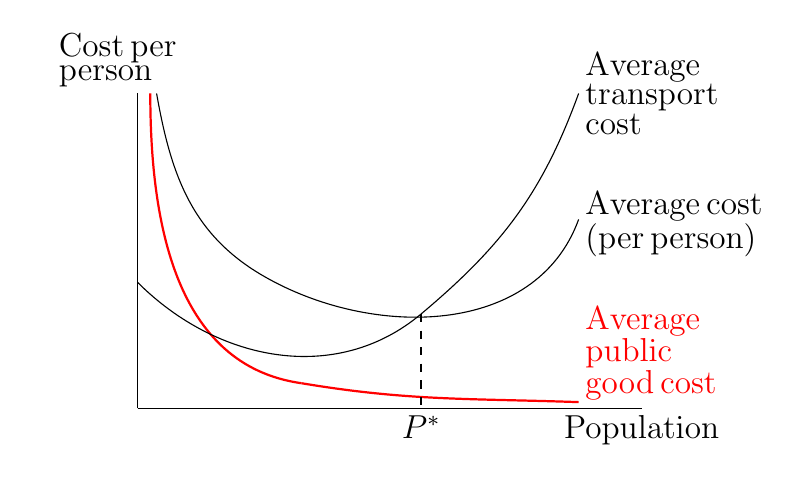
\begin{tikzpicture}[scale=0.8]
\tiny
\draw (0,0) -- (8,0) node [below] {\large Population};
\draw (0, 0) -- (0,5) node [above, text width=2cm] {\large Cost per person};
\draw [red, thick] (0.2,5) to [out=270,in=172] (2.6,0.4);
\draw[red, thick] (2.6,0.4) to [out=350.5,in=178] (7,0.1);
\node [red, above=.3cm, right, text width=2cm] at (7,0.5) {\large Average public good cost};
\draw (0.3,5) to [out=280,in=150] (2,2.1);

\draw (2,2.1) to [out=330,in=250] (7,3);
\node [above right, text width=2.5cm] at (7,2.3) {\large Average cost\newline (per person)};
%\draw (0,2) to [out=340,in=200] (7,1.8);
%\node [right] at (7,1.8) {$AVC$};

\draw (0,2) to [out=315, in=220] (4.5,1.5) to [out=40,in=250] (7,5);
\node [right, text width=2cm] at (7,5) {\large Average transport cost};

\draw [dashed, thick] (4.5,1.5)--(4.5,0)node[below]{\large $P^*$};
\end{tikzpicture}
\caption{Optimal city size with a public good}
\end{figure}


    %%%%%%%%%%%%%%%%%%%%%%%%%%%%%%% END STUFF

 % Has errors

% \documentclass[notes]{beamer}
\usepackage{graphics}
\usepackage{url}
\usepackage {amssymb}
\usepackage{xcolor}
\usepackage{tikz}
\usetikzlibrary{positioning}
\usetikzlibrary{shadows}
\usetikzlibrary{arrows,automata,shapes,calc}
%\usepackage{enumitem}
%\usepackage{onimage}
 \usepackage{standalone}

\usecolortheme{crane}
\parskip=10pt plus 1pt


\begin{document}
  \title{Ricardo, Rent, and Roemer: \\Class and exploitation in the financialized city}

%\author[Dr. David Robinson,Kirsten Wright]{Dr. David Robinson\inst{Laurentian University}  \and Kirsten Wright\inst{University of Waterloo} }

\author{Dr. David Robinson\hspace{30pt}Kirsten Wright\\
           Laurentian University, University of Waterloo}%\\
%             \ \\
%           \small Prepared for the Annual Conference of the \\
%           \small  Canadian Economic Association, June 3-5, 2021}
 
\def\defn#1{{\color{red} #1}}

 %\logo\pgfdeclareimage[height=0.5cm]{INORDlogo\_April2012-eps-converted-to.pdf}{tu-logo}


%% 
%\usepackage{graphicx}
%% \usepackage[table]{xcolor}
%
%\begin{document}
\begin{frame}
\titlepage
\end{frame}
%%%%%%%%%%%%%%%%%%%%%%%%%%%%%%%%%%%%%%%%%%%%%%%%%%%% FRAME

\begin{frame}\frametitle{Outline}
\tableofcontents
\end{frame}


\section{A Question}%%%%%%%%%%%%%%%%%%%%%%%%%%% FRAME

\begin{frame}\frametitle{}

\begin{itemize}
\item Housing prices keep going up
\item Young people can't buy houses.\vspace{.5cm}

\hspace{2cm} {\Large Its just a bubble? } \vspace{.5cm}\pause

\item The global population is moving to cities

\item technological change is accelerating
\item the global wealth  distribution is getting worse

\end{itemize}\vspace{.5cm}

\hspace{2cm}{\Large Are all these economic features }

\hspace{2cm} {\Large of our modern world related?}\vspace{.5cm}\pause

\hspace{6cm}We think so.

\end{frame}
\section{The Model and it's History} %%%%%%%%%%%%%%%%%%%%%%%%%%%%%%%%%%%%%% FRAME
\begin{frame}\frametitle{A note:}
This is a tricky paper to present. We have been expecting an audience with distinguished economists, green activists, undergraduate economics students, and possibly academics from other fields,  and even some Marxists-at-large.

It is a fairly technical paper using a lot of tricks of the trade, and we will play that part down so we can focus on the story

We are combining ideas about the source of income for various classes from Ricardo, and Marx with a modern growth models and and standard urban model. %He  focussed on the exploitation of the  rising class of industrial workers, but his thinking, unlike Ricardo's, was  much more dynamic.
\end{frame}
%%%%%%%%%%%%%%%%%%%%%%%%%%%%%%%%%%%%%%%%%%%%%%%%%%% FRAME
\begin{frame}\frametitle{The model}
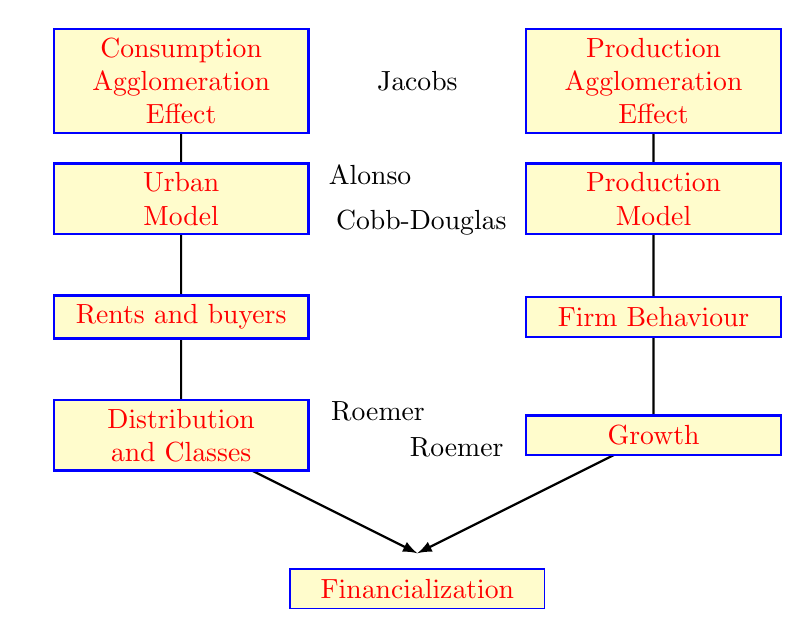
\begin{tikzpicture}[scale=.5]
%\tikzset{every node/.style={red, draw=blue, fill=yellow!20, minimum size=0.5cm, text width =3cm, align = center},}	
\def \left {6}
\def \right {-\left}
\def \top {10}
\def \skip {-3}
\node at (0,\top) {Jacobs};
\node at (-1.2,{\top+.8*\skip}) {Alonso};
\node at (0.1,{\top+1.2*\skip}) {Cobb-Douglas};
\node at (-1,{\top+2.8*\skip}) {Roemer};
\node at (1,{\top+3.1*\skip}) {Roemer};
%\node at (0,{\top+4.3*\skip}){Financialization};

\tikzset{every node/.style={red, draw=blue, fill=yellow!20, minimum size=0.5cm, text width =3cm, align = center},}	
\draw[-latex,  thick, to path={-| (\tikztotarget)}, outer sep=2pt](\left,\top)node {Production \\ Agglomeration\\ Effect} -- ( \left,{\top+\skip})node {Production \\ Model}--( \left,{\top+2*\skip})node {Firm Behaviour} -- ( \left,{\top+3*\skip})node{Growth}-- (0,{\top+4*\skip} ); 

\draw[-latex,  thick, to path={-| (\tikztotarget)}](\right,\top)node {Consumption \\ Agglomeration\\ Effect} --( \right,{\top+\skip})node {Urban \\ Model}--( \right,{\top+2*\skip})node {Rents and buyers} -- ( \right,{\top+3*\skip})node{Distribution and Classes}-- (0,{\top+4*\skip} ); 
\node at (0,{\top+4.3*\skip}){Financialization};

\end{tikzpicture}
\end{frame}

%%%%%%%%%%%%%%%%%%%%%%%%%%%%%%%%%%%%%%%%%%%%%%%%%%%% FRAME
%\begin{frame}\frametitle{}
%
%
%%The point here is that Marx identified the dominant economic transformation of his time and produced a theory of how it evolved in historical time.  Marx took over Hegel's teleological account of history and developed a materialist theory ( I would call it an \textbf{economic} theory) of historical development class relations and distribution.
%
%Neither Marx nor Ricardo were particularly good at calculus, and they didn't have the tools of modern economics, so they did not talk about classes the way a modern economist would. On the other hand, and most economists are not very good at history and especially class issues, so the modern framework has not been applied to the recent transformation of the economic base.
%
%That's what this paper is trying to do. 
%
%
%\end{frame}
%%%%%%%%%%%%%%%%%%%%%%%%%%%%%%%%%%%%%%%%%%%%%%%%%%%% FRAME
\begin{frame}\frametitle{Production, rent, surplus labour, and exploitation}%A run through the history of economic thought to collect some tools}
% These are the big names in classical rent theory
\begin{itemize}
\item Ricardo of had two factors of production: land and labour. 
\textbf{\textit {The class that owned all the land earned land rents: exploited the peasants labour.}}

\item  In the industrial revolution, which Marx focussed on, English landowners replaced peasants with sheep creating a pool of ``free labour'' that was cheap. %Das Kapital. Kritik der politischen Ökonomie,  1867–1883)

\textbf{\textit {The class that owned all the produced capital needed for industrial production earned land rents - (Marx called it surplus value): exploited the free labour.}}

\item After Marx, Henry George, identified something like Ricardian land rents as the basis of exploitation.
%\begin{quotation}{\tiny \noindent by far ``the most famous American economic writer'' and ``author of a book which probably had a larger world-wide circulation than any other work on economics ever written''}
%\end{quotation}
\item Roemer analyzed class and exploitation in a multi-factor GE economy. 
\end {itemize}
\end{frame}

%%%%%%%%%%%%%%%%%%%%%%%%%%%%%%%%%%%%%%%%%%%%%%%%%%%% FRAME
\begin{frame}\frametitle{}

\begin{itemize}  
\item After Ricardo, Marx, and George, more mathematical economists described production with  ``Functions'', such such as the Cobb-Douglas  form (1927)
\begin{eqnarray*}
Y=& f(Land, Labour, Capital) \\ 
Y=&L^0 K^{\textcolor{red}{\alpha}} N^{\textcolor{red}{\beta}}
\end{eqnarray*}


\item The values of $\alpha$ and $\beta$. are very important. 

If $\alpha+\beta >1$ a single firm takes over the world.  

If $\alpha+\beta <1$ a large city has competitive firms and, as Marshall pointed out, zero profits in equilibrium*.

\pause

% Marx and Ricardo would have understood this - they both grasped diminishing marginal returns, but the techniques had not been developed   (Qualifications: Von Thunen, The Isolated State (1826)  Cournot   Researches on the Mathematical Principles of the Theory of Wealth (1838)  

\item \textbf{\color{red}Technical Discovery:} production was increasing more rapidly than the combined supply of land labour and capital predicted. 

\item Solow introduced a term, $A(t)$,  called ``total factor productivity.'' 

\[Y= \textcolor{red} {A(t)} L^0 K^\alpha N^\beta\]

\end {itemize}
\end{frame}

%%%%%%%%%%%%%%%%%%%%%%%%%%%%%%%%%%%%%%%%%%%%%%%%%%%% FRAME
\begin{frame}\frametitle{}
\begin{itemize} 


\item In the 1960's  growth economists fiddled with this idea calling it things like ``labour augmenting technological change,'' ``human capital,'' ``learning,'' ``technology,''

\item They realized that human skills, knowledge, institutions,  and social organization  
are factors of production like labour, land and capital.  \vspace{1cm}

In Endogenous Growth theories, ``$A$'' depends on education spending, investment in invention, investment in previous production. 

These are things that can be influenced by government policy.



\end {itemize}
\end{frame}

%%%%%%%%%%%%%%%%%%%%%%%%%%%%%%%%%%%%%%%%%%%%%%%%%%%% FRAME
\begin{frame}\frametitle{The city as the source of productivity}
\begin{itemize}

\item In 1985 Jane Jacobs published \textbf{Cities and the Wealth of Nations}, arguing that urban agglomeration itself accounted for a great deal of the increase in productivity that mystified the growth theorists. In $N$ is urban population,

\[Y=  \textcolor{red} {A(N)}K_i^\alpha N_i^\beta\]

\item The difference between total labour $N$ and the labour used by an individual firm  $N_i$  matters. The firm can't take credit for increasing productivity. It is a social product.

\item \textbf{This raises the question, ``Who should get that benefit?''}
%\item In 1990 John Porter kicked off a project that led to cluster theory and a a focus on  agglomeration economies.

\end {itemize}

\end{frame}


\section{The Urban Model}%%%%%%%%%%%%%%%%%%%%%%%%%%%%%%%%%%%%%%%%%% FRAME
% \begin{frame}\frametitle
{A parallel development of rent theory}
\begin{itemize} 

\item In 1964, William Alonso published \textbf{Location and Land Use}, in which he defined a model %of the formation of land rent in urban environments. He 
that specifically linked urban agglomeration to land rents and this became the central model in modern urban economics.

\item We use an \textbf{Alonso-Jacobs model} to explore the distribution surplus value.
\end {itemize}
% \end{frame}

%%%%%%%%%%%%%%%%%%%%%%%%%%%%%%%%%%%%%%%%%%%%%%%%%%%% FRAME
\begin{frame}\frametitle{Alonso's Circular City}
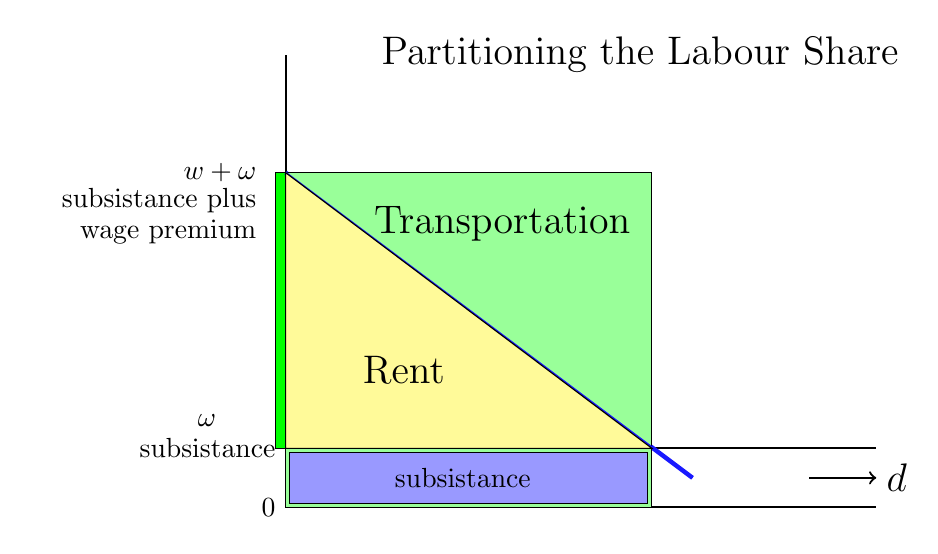
\begin{tikzpicture}[scale=.5]
\def\bndmax{5}        %https://tex.stackexchange.com/questions/68462/filling-a-complex-region-with-tikz
\def\bndmin{0.2}
\def \n {10}  % height of y axis
\def \d {15}  % length  of x axis
\def \t {.75}  %  cost of transportation per unit x
\def \th {1}   %
\def \w {7}    %  wage premium
\def \om{1.5}%  omega =rural wage Zero for urban population
\def \azero{2}
\def \aprime {-.0}	
\tikzset{func/.style={thick,color=blue!90}}	

% FIRST FIGURE just axes
\draw [thick] (0,-\om) --(\d,-\om);  			% Zero for rural population
\draw [thick] (0,-\om)node[left]{$0$} --(0,\n);	% Y axis
%\node at (0,\n+0.5){\large$Rent$};

\draw [thick] (0,0)node[left]{subsistance}--(\d,0);
\node a t(-2,.7) {$\omega$};
\node[left=.25] at (0,\w){$w+\omega$};
\node[left=.25] at (0,\w-.7){subsistance plus};
\node[left=.25] at (0,\w-1.5){wage premium};	

%\foreach \xi in {0,..., \n} \draw (\xi,0)--(\xi,-.1)node[below=1]{\small$\xi$};
%\foreach \yi in {1,...,\n} \draw (0,\yi)--(-.1,\yi)node[left]{$\yi$};
%\foreach \i in {1,4,9,16} {
\node at (7,-\om/2){people scattered uniformly across the land  };

%SECOND FIGURE WITH AGGLOMERATION WAGE
\pause %  add urban production and net wage
\draw[fill=white, white] (0.1,-0.1) rectangle (14,-\om+.1);
\draw [fill=green] (-.25, 0) rectangle(.25, \w);
\node[right] at  (.25, \w/2){Added Productivity};
\node[right, text width = 3cm] at  (10,9){Where does the increase in productivity come from?};
\draw [ thick, ->](13.3,-\om/2)--(15, -\om/2)node [right] {\Large $d$};

%  THIRD FIGURE  add wage profile
\pause
\node[right, white, fill=white,  text width = 3cm] at  (10,9){Where does the increase in productivity come from?};
\draw[func, domain=0:\w/\t+1,ultra thick] plot [samples=200] (\x,{\w-\t*\x}); %Net wageprofile  for 
\node[right, white, fill=white] at  (.25, \w/2){Added Productivity};
\node[right, fill=white, text width =3.5cm ] at  (1, \w/2){Declining wage  net \\of transportation\\ costs $T(d)$ };

%   FOURTH FIGURE     commuters
\pause
\draw[fill=blue!40] (0.1,-0.1) rectangle (9.2,-\om+.1);
\node at (4.5,-\om/2){commuters};

%   FOURTH FIGURE    wage bill
\pause %add total new value
\draw[fill=green!40] (0,-\om) rectangle(9.30,\w);% new product
\node at (4.5,\w/2){\Large urban wage bill};

%%   FIFTH FIGURE   distribution
\pause
\node at (9,\n){\Large Partitioning the Labour Share};

\draw[fill=green!40] (0,-\om) rectangle (9.30,\w);% new product repeat
\draw[func, domain=0:\w/\t+1] plot [samples=200] (\x,{\w-\t*\x}); %rent profile
\draw[fill=blue!40] (0.1,-0.1) rectangle (9.2,-\om+.1);
\node at (4.5,-\om/2){subsistance};
\draw[fill=yellow!40] (0.,0.) -- (0,7)--(9.30,0.)--cycle;% Rent \w-.2
\node at (3.,2){\Large Rent}; 		%Rent 
\node at (5.5,5.7){\Large Transportation};
 \end{tikzpicture}
\end{frame}

\section{Distributional issues}%%%%%%%%%%%%%%%%%%%%%%%%%%%%%%%%%%%%%%%%%% FRAME
\begin{frame}\frametitle{Who gets the rent?}

\begin{itemize}
\item It is capitalized into land values - 
\item The original land owners get the increase in land value. Why should they?
\item They realize the value if they sell the property.
\item New owners MAY get rents from future productivity increases.\vspace{1cm}
\end {itemize}
\end{frame}
%%%%%%%%%%%%%%%%%%%%%%%%%%%%%%%%%%%%%%%%%%%%%%%%%%%% FRAME
\begin{frame}\frametitle{Two notes}

\begin{itemize}
\item Property taxes take some of the value for the community. How much is the community entitled to?

\item In 1977, Joseph Stiglitz  proved the "Henry George Theorem" that said urban land rents would be all you needed to pay for public goods that make a city attractive. 

\item A 100\% tax on capital gains in land is the logical consequence
% My note on this is cited in the wikipedia article on the Henry George Theorem!
\end {itemize}


\end{frame}

%%%%%%%%%%%%%%%%%%%%%%%%%%%%%%%%%%%%%%%%%%%%%%%%%%%% FRAME
\begin{frame}\frametitle{Class Analysis: The city so far.}
\begin{itemize}
\item Before  anyone sells their property there are two classes: Capitalists and workers.
\item when a property owner sells the property they  own capital, which mean s they receive an income share of future wages: They are members of an intermediate class of small capitalists.
\item They may invest and continue working or work less and live in part off of the labour of others.  
\item John Roemer in \textbf{A General Theory of Exploitation and Class} (1982) offers  formal definitions of `exploited' and `exploiter'. This group falls in both  categories and can be classified as neither

\end {itemize}

\end{frame}
\section{Consumption Amenities} %%%%%%%%%%%%%%%%%%%%%%%%%%%%%%%%%%%%%%% FRAME
\begin{frame}\frametitle{Adding consumption amenities}
There can be agglomeration benefits of urban life - $ \textcolor{red}{\mathcal{A}(N,d)}$
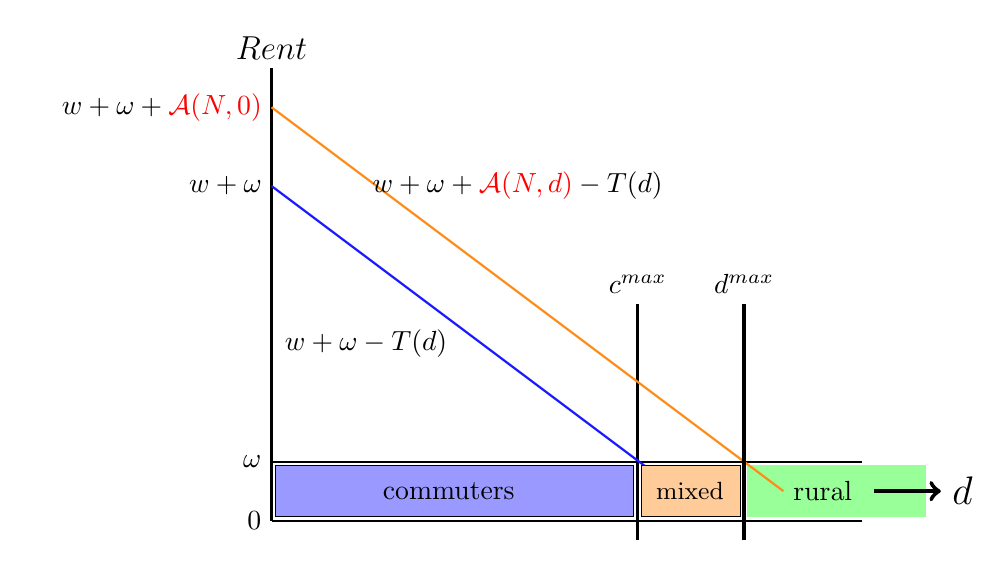
\begin{tikzpicture}[scale=.5]
\def\bndmax{5}        %https://tex.stackexchange.com/questions/68462/filling-a-complex-region-with-tikz
\def\bndmin{0.2}
\def \n {10}  % height of y axis
\def \d {15}  % length  of x axis
\def \t {.75}  %  cost of transportation per unit x
\def \th {1}   %
\def \w {7}    %  wage premium
\def \om{1.5}%  omega =rural wage Zero for urban population
\def \azero{2}
\def \aprime {-.0}	
\tikzset{func/.style={thick,color=blue!90}}	

\draw [thick] (0,-\om) --(\d,-\om);  	% Zero for rural population
\draw [thick] (0,-\om)node[left]{$0$} --(0,\n);			% Zero for urban population
\node at (0,\n+0.5){\large$Rent$};

\draw [thick] (0,0)node[left]{$\omega$}--(\d,0);
\node[] at ({\d+.5},-\om/2) {\Large $d$};
%\foreach \xi in {0,..., \m} \draw (\xi,0)--(\xi,-.1)node[below=1]{\small$\xi$};
%\foreach \yi in {1,...,\n} \draw (0,\yi)--(-.1,\yi)node[left]{$\yi$};
%%\foreach \i in {1,4,9,16} {


\draw [very thick](9.3,-2)-- ++ (0,6)node[above]{$c^{max}$};;

% solid color for commuters
\draw[fill=blue!40] (0.1,-0.1) rectangle (9.2,-\om+.1);
% Net wageprofile  for commuters
\draw[func,domain=0:\w/\t+1] plot [samples=200] (\x,{\w-\t*\x});
	%	\draw[func,domain=0:\m, dashed] plot [samples=200] (\x,{\w+\azero-\th*\x+\aprime*\x});
\node[left] at (0,\w){$w+\omega$};	
\node at (2.4,3.){$w+\omega-T(d)$};
\node at (4.5,-\om/2){commuters};

% solid color for transition
\draw[fill=orange!40] (9.4,-0.1) rectangle (11.9,-\om+0.1);
	\node[text width=2] at (9.84,-\om/2){\small mixed};
\draw[fill=green!40, green!40] (12.1,-0.1) rectangle (16.6,-\om+0.1);
\node at (14,-\om/2){rural};
\draw [ ultra thick, ->](15.3,-\om/2)--(17, -\om/2)node [right] {\Large $d$};
% Net amenity profile  for commuters
	\tikzset{func/.style={thick,color=orange!90}}	
		\draw[func,domain=0:\d-2] plot [samples=200] (\x,{\w+\azero-\t*\x+\aprime*\x});
	\node[left] at (0,{\w+\azero} ){$w+\omega + \textcolor{red}{\mathcal{A}(N,0)}$};
	\node at (6.25,7 ){$w+\omega +\textcolor{red}{\mathcal{A}(N,d)}-T(d)$};

	\draw [very thick](12,-2)-- ++ (0,6)node[above]{$d^{max}$};
 
 \end{tikzpicture}
% ****   notice mixed: they get benefits don't work and pay rent. ***Rent is higher!!
\end{frame}

%%%%%%%%%%%%%%%%%%%%%%%%%%%%%%%%%%%%%%%%%%%%%%%%%%%% FRAME
\begin{frame}\frametitle{Who gets the amenities?}
\begin{itemize}
\item They go to property owners 

\item When owners sell they capture the capitalized  value of the amenity

\item Tenants pay rent that captures the value of the amenity for the land owner. 


\end{itemize}



\end{frame}


\section{The evolution of the Urban System}%%%%%%%%%%%%%%%%%%%%%%%%%%%%%%%%%%%%%%%% FRAME
\begin{frame}\frametitle{Growth andPrices }

\begin{itemize}
\item If wages do not rise, the new owners do not get any of the captalized value of the rent

\item  Will the urban wage premium rise? 
	\begin{quotation}
	In our model, capital captures some of the agglomeration benefits in production. It earns an excess return or super-profit. This attracts more capital, which demands more labour. This pushes up the wage to attract more workers. 
	\end{quotation}
	
\item More labour increases agglomeration effect, resulting in more investment and  more growth. 
\item capital will compete for the \textbf{perpetual capital gain from urban  land} 


\pause
\item Therefore \textcolor{red}{land prices rise as long as there is a  supply of workers}
\end{itemize}


\end{frame}
%%%%%%%%%%%%%%%%%%%%%%%%%%%%%%%%%%%%%%%%%%%%%%%%%%%% FRAME
\begin{frame}\frametitle{Urban land becomes a \textbf{speculative asset} }
So who buys speculative assets?
 \pause
 
\begin{itemize}
\item {\Large Returns on capital are higher for wealthy investors}
\item Why? People with higher wealth get 
	\begin{enumerate}
	\item lower borrowing costs
	\item higher borrowing limits,  allowing more leverage
	\item professional investment advice
	\end{enumerate}
\item People with higher wealth may be less risk-averse 
\item People with higher wealth are generally more liquid 
\item People with higher wealth may have more confidence about long term investments
\end{itemize}

\Large The wealthy will bid more than the less wealthy.

\tiny This contradicts a standard assumption in modelling


\end{frame}


%%%%%%%%%%%%%%%%%%%%%%%%%%%%%%%%%%%%%%%%%%%%%%%%%%% FRAME
\begin{frame}\frametitle{Who will the new owners be?}


\begin{enumerate}
\item  land prices rise continually
\item urban land becomes a speculative asset
\item Ownership of urban land is increasingly concentrated in the wealth holding class as a financial asset 
\item new workers are shut out of the land market.
\end{enumerate}



\end{frame}
%%%%%%%%%%%%%%%%%%%%%%%%%%%%%%%%%%%%%%%%%%%%%%%%%%% FRAME

\begin{frame}\frametitle{Conclusions}
\begin{enumerate}
\item attempts to make home ownership for new entrants affordable can only bid up prices 
\item The fundamental problem is private ownership of land, which allows individuals and capital to capture the social surplus value generated by agglomeration.
\end{enumerate}



\end{frame}

%%%%%%%%%%%%%%%%%%%%%%%%%%%%%%%%%%%%%%%%%%%%%%%%%%%%% FRAME
\begin{frame}\frametitle{}
%\includegraphics[scale=1]{x.jpg}

\end{frame}

\end{document}


%%%%%%%%%%%%%%%%%%%%%%%%%%%%%%%%%%%%%%%%%%%%%%%%%%%% FRAME
\begin{frame}\frametitle{}
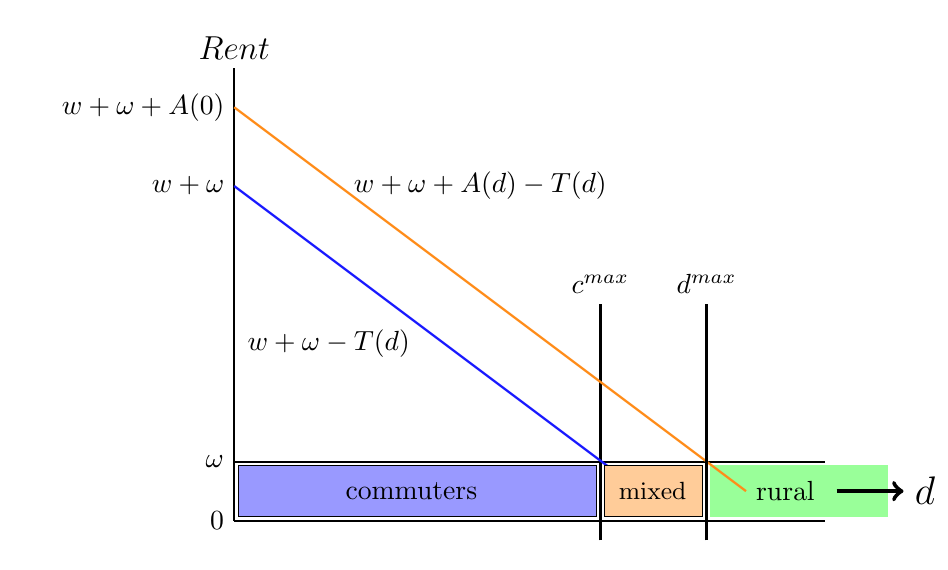
\begin{tikzpicture}[scale=.5]
\def\bndmax{5}        %https://tex.stackexchange.com/questions/68462/filling-a-complex-region-with-tikz
\def\bndmin{0.2}
\def \n {10}  % height of y axis
\def \d {15}  % length  of x axis
\def \t {.75}  %  cost of transportation per unit x
\def \th {1}   %
\def \w {7}    %  wage premium
\def \om{1.5}%  omega =rural wage Zero for urban population
\def \azero{2}
\def \aprime {-.0}	
\tikzset{func/.style={thick,color=blue!90}}	

\draw [thick] (0,-\om) --(\d,-\om);  	% Zero for rural population
\draw [thick] (0,-\om)node[left]{$0$} --(0,\n);			% Zero for urban population
\node at (0,\n+0.5){\large$Rent$};

\draw [thick] (0,0)node[left]{$\omega$}--(\d,0);
\node[] at ({\d+.5},-\om/2) {\Large $d$};
%\foreach \xi in {0,..., \m} \draw (\xi,0)--(\xi,-.1)node[below=1]{\small$\xi$};
%\foreach \yi in {1,...,\n} \draw (0,\yi)--(-.1,\yi)node[left]{$\yi$};
%%\foreach \i in {1,4,9,16} {


\draw [very thick](9.3,-2)-- ++ (0,6)node[above]{$c^{max}$};;

% solid color for commuters
\draw[fill=blue!40] (0.1,-0.1) rectangle (9.2,-\om+.1);
% Net wageprofile  for commuters
\draw[func,domain=0:\w/\t+1] plot [samples=200] (\x,{\w-\t*\x});
	%	\draw[func,domain=0:\m, dashed] plot [samples=200] (\x,{\w+\azero-\th*\x+\aprime*\x});
\node[left] at (0,\w){$w+\omega$};	
\node at (2.4,3.){$w+\omega-T(d)$};
\node at (4.5,-\om/2){commuters};

% solid color for transition
\draw[fill=orange!40] (9.4,-0.1) rectangle (11.9,-\om+0.1);
	\node[text width=2] at (9.84,-\om/2){\small mixed};
\draw[fill=green!40, green!40] (12.1,-0.1) rectangle (16.6,-\om+0.1);
\node at (14,-\om/2){rural};
\draw [ ultra thick, ->](15.3,-\om/2)--(17, -\om/2)node [right] {\Large $d$};
% Net amenity profile  for commuters
	\tikzset{func/.style={thick,color=orange!90}}	
		\draw[func,domain=0:\d-2] plot [samples=200] (\x,{\w+\azero-\t*\x+\aprime*\x});
	\node[left] at (0,{\w+\azero} ){$w+\omega +A(0)$};
	\node at (6.25,7 ){$w+\omega +A(d)-T(d)$};

	\draw [very thick](12,-2)-- ++ (0,6)node[above]{$d^{max}$};
%\node at(-.8,2) [left]{base $2^1=$};
%\node at(-.8,1) [left]{$2^0=$};
%\draw[dotted] (0,2)--(1,2)--(1,0); 
 \end{tikzpicture}



\end{frame}
%%%%%%%%%%%%%%%%%%%%%%%%%%%%%%%%%%%%%%%%%%%%%%%%%%%% FRAME
\begin{frame}\frametitle{}
\includegraphics[size=1]{Thats_all_folks.svg}

\end{frame}

%%%%%%%%%%%%%%%%%%%%%%%%%%%%%%%%%%%%%%%%%%%%%%%%%%%% FRAME
\begin{frame}\frametitle{}
\begin{itemize}
\item 
\end{itemize}
\end{frame}

%%%%%%%%%%%%%%%%%%%%%%%%%%%%%%%%%%%%%%%%%%%%%%%%%%%% FRAME
\begin{frame}\frametitle{}



\end{frame}
%%%%%%%%%%%%%%%%%%%%%%%%%%%%%%%%%%%%%%%%%%%%%%%%%%%% FRAME
\begin{frame}\frametitle{}
\begin{itemize}
\item 
\end{itemize}
\end{frame}
%%%%%%%%%%%%%%%%%%%%%%%%%%%%%%%%%%%%%%%%%%%%%%%%%%%% FRAME
\begin{frame}\frametitle{}



\end{frame}
%%%%%%%%%%%%%%%%%%%%%%%%%%%%%%%%%%%%%%%%%%%%%%%%%%%% FRAME
\begin{frame}\frametitle{}



\end{frame}
%%%%%%%%%%%%%%%%%%%%%%%%%%%%%%%%%%%%%%%%%%%%%%%%%%%% FRAME
\begin{frame}\frametitle{}



\end{frame}
%%%%%%%%%%%%%%%%%%%%%%%%%%%%%%%%%%%%%%%%%%%%%%%%%%%% FRAME
\begin{frame}\frametitle{}



\end{frame}
%%%%%%%%%%%%%%%%%%%%%%%%%%%%%%%%%%%%%%%%%%%%%%%%%%%% FRAME
\begin{frame}\frametitle{}



\end{frame}
%%%%%%%%%%%%%%%%%%%%%%%%%%%%%%%%%%%%%%%%%%%%%%%%%%%% FRAME
\begin{frame}\frametitle{}



\end{frame}
%%%%%%%%%%%%%%%%%%%%%%%%%%%%%%%%%%%%%%%%%%%%%%%%%%%% FRAME
\begin{frame}\frametitle{}



\end{frame}

%%%%%%%%%%%%%%%%%%%%%%%%%%%%%%%%%%%%%%%%%%%%%%%%%%%%    END
\end{document} % BEAMER PRESENTATION

\bibliographystyle{plain}
\cleardoublepage % This is needed if the "book" document 
\phantomsection
\renewcommand*{\bibname}{References}
\addcontentsline{toc}{chapter}{\textbf{References}}
\bibliography{thesis-bib.bib}
% \bibliography{bib_resilience,bib_housing}

\printglossary
\cleardoublepage
\phantomsection		% allows hyperref to link to the correct page





 
 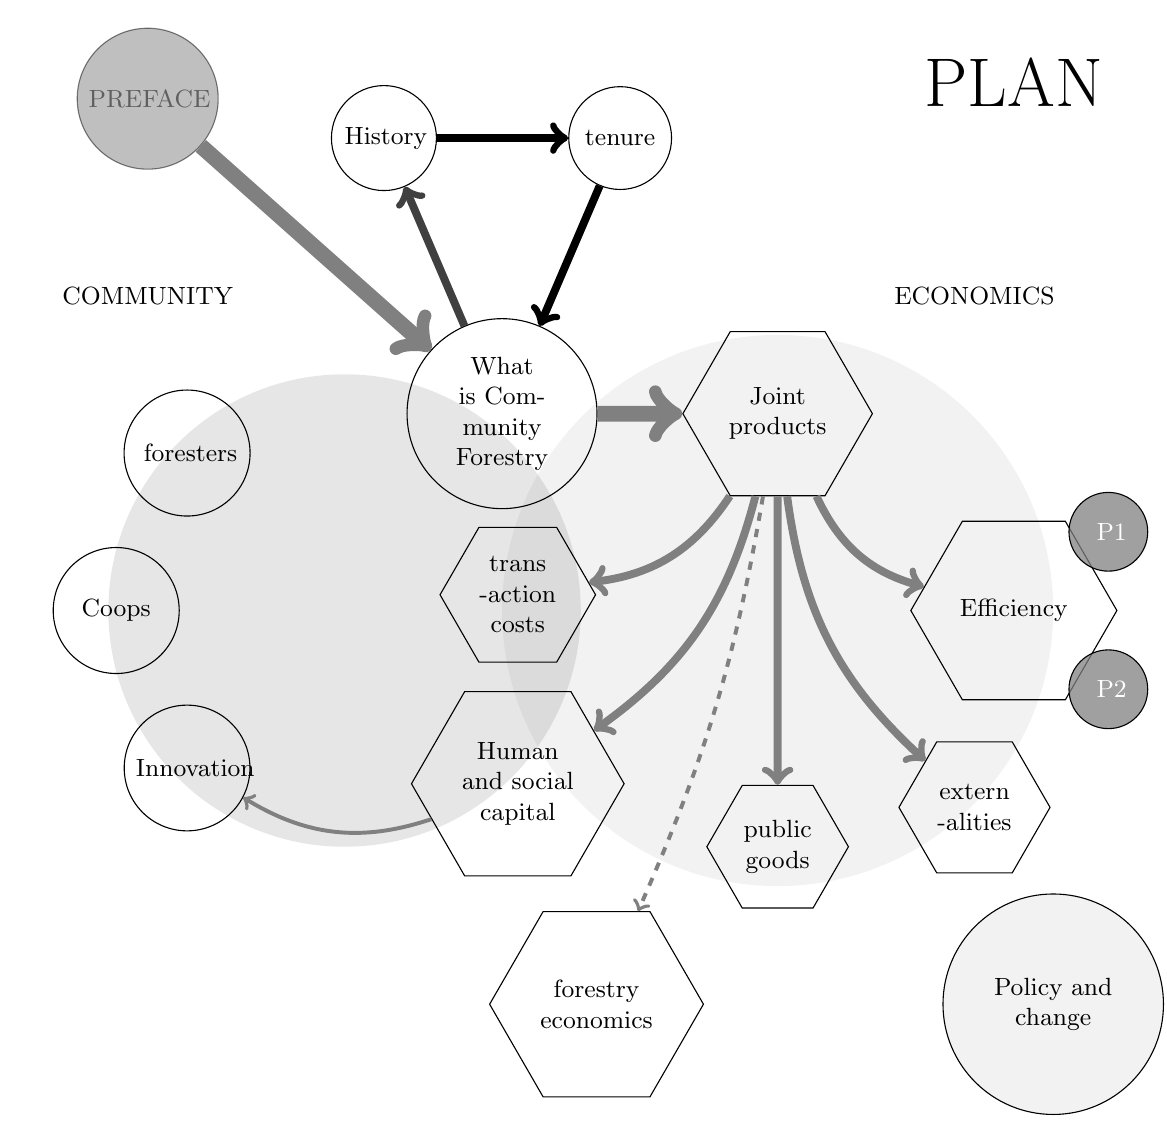
\begin{tikzpicture}%[scale=.8]
    \tikzstyle{every node}=[font=\small]
%\draw[help lines,step=.5] (0,-11) grid (11,11);

\coordinate (aa) at (-1.5,7.5);%PREFACE
\coordinate (a) at (-1,10);%
 \coordinate (b) at (1.5,7); %history
\coordinate (c) at (6,10); %
\coordinate (d) at (9,9);%
\coordinate (ee) at (-4,7);%
  \coordinate (e) at (-1.5,5); %Community label
\coordinate (f) at (9.5,7.7); %???    PLAN
\coordinate (g) at (9,5); %Economics label
\coordinate (h) at (4.5,7);%tenure
\coordinate (ii) at (-4,4);%
   \coordinate (i) at (1,4);  
\coordinate (j) at (3,3.5);%whatis
\coordinate (k) at (6,4);%
 \coordinate (l) at (6.5,3.5);%joint
\coordinate (mm) at (-1.9,1);%coops
 \coordinate (m) at (1,1);%community grey circle
  \coordinate (n) at (3,1); %
  \coordinate (o) at (9.5,1); %efficiency
				 \coordinate (oo) at (6.5,1);%
				  \coordinate (o1) at (10.7,2);	 \coordinate (o2) at (10.7,0);%Propositions
\coordinate (p) at (9,-1.5);%externalities
				
\coordinate (qq) at (-4,-2);
\coordinate (q) at (-1,-1);%innovation
 \coordinate (r) at (3.2,1.2);%trans
  \coordinate (s) at (3.2,-1.2);%capital
 \coordinate (t) at (6.5,-2);%pubgoods
\coordinate (AA) at (-2,-5);%
 \coordinate (A) at (1,-5);%
\coordinate (B) at (3.7,-4); %
\coordinate (C) at (4.2,-4);%forestryEC
\coordinate (D) at (-1,3);%foresters
\coordinate (EE) at (-1,-8); \coordinate (E) at (1,-8); \coordinate (F) at (3,-8); \coordinate (G) at (6,-8); \coordinate (H) at (10,-4);%Policy
\coordinate (II) at (-4,-11);  \coordinate (I) at (1,-11); \coordinate (J) at (3,-11); \coordinate (K) at (6,-11); \coordinate (L) at (10,-11);
%\coordinate (M) at (coordinate); \coordinate (N) at (coordinate); \coordinate (O) at (coordinate); \coordinate (P) at (coordinate);
%\coordinate (Q) at (coordinate); \coordinate (R) at (coordinate); \coordinate (S) at (coordinate); \coordinate (T) at (coordinate);
% \fill[red, fill opacity=.8] (0,0) circle (4cm);
\fill [gray, fill opacity=0.2] (m) node [text width=2cm, black, opacity=1] 				(community)	{} circle (3cm);
\fill [gray, fill opacity=0.1] (oo)  node [text width=2cm, align=left, black, opacity=1] 		(econ) {} circle (3.5cm);
\node at (e) [ ] 		(comLtabel) {COMMUNITY};
\node at (g) [ ] 		(ecLabel) {ECONOMICS};
				%\draw (0,3.2,1) node [text width=1.5cm, text centered] {$Economics$};
			%\draw [fill=red, fill opacity=0.3]  (aa) node [ text width=2cm, black, opacity=1] 									(preface)		{PREFACE: Why, claims} circle (1.4cm);
\node [circle, draw,  fill=gray, opacity=.5,, text width=1.5cm] at			 (aa) 		(preface)		{PREFACE};
\node [] at			 (f) 		(plan)		{\Huge PLAN};
			%\draw [fill=blue, fill opacity=0.35] (b)node [text width=2cm, align=center, black, opacity=1] 			(history){History: New is Old} circle (1.2cm);
\node[circle, draw, text width=1cm, align=center, black, opacity=1]at 	(b)(history){History} ;
			%\draw [fill=pink, fill opacity=0.5] 		(h) node [text width=2cm, black, opacity=1] 								(tenure) 	{\color{black}tenure} circle (1.2cm);
\node[circle, draw,  text width=1cm, align=center, black] at 				(h) (tenure) 	{tenure} ;
\node[circle, draw,  text width=1.5cm, align=center]at							 (j) (whatis) 	{\color{black}What is Community Forestry} ;
\node[regular polygon, regular polygon sides=6, draw, align=center]at (l) (joint) 	{\color{black}Joint\\  products} ;


%\node[circle, draw,  text width=2cm, align=center]at (h) (tenure) 	{\color{black}tenure} ;

%\draw [fill=red, fill opacity=0.5] (j) node [text width=2cm, black, opacity=1] 												(whatis)		{What is Community Forestry}circle (1.4cm);
%\draw [fill=orange, fill opacity=0.5] 	(l) node [text width=2cm, black, text opacity=1] 	               		(joint)	{Joint products}											 circle (1.2cm);
%\draw [fill=green, fill opacity=0] (1,5)node [text width=2cm,red, opacity=1] {Policy and change} circle (1.4cm);
%\draw (q) node [text width=1.3cm, align=center, black, opacity=1] (small)	 {Innovation} circle (1.1cm);
\node[circle, draw,  text width=1.3cm, align=center] at							 (q) (small)	 {Innovation} ;

\draw 	(mm) node [text width=1.3cm, align=center, black, opacity=1] 	(coops) 	{Coops} circle (.8cm);
%\draw [fill=orange, fill opacity=0.5] 	(s) node [text width=2cm,  align=center, black, text opacity=1] (capital) {Human \\and social \\capital} circle (1.2cm);
\node[regular polygon, regular polygon sides=6, draw, align=center] at (s) (capital) {Human \\and social \\capital} ;
%\draw [fill=gray, fill opacity=0.5] 			(o) node [text width=2cm, black, text opacity=1] 						(efficiency)	{Efficiency} circle (1.2cm);
\node[regular polygon, regular polygon sides=6, draw, align=center] at (o) (efficiency)	{Efficiency};
\draw [fill=gray, fill opacity=0.75] (o1) node [text width=.3cm, white, text opacity=1] (	P1)  {P1} 		circle (.5cm);
\draw [fill=gray, fill opacity=0.75] (o2) node [text width=.3cm, white, text opacity=1] (P2) {P2} 			circle (.5cm);

%\draw [fill=orange, fill opacity=0.5] (p) node [text width=2cm, black, opacity=1]					(externalities)	 {externalities} 			circle (1.2cm);
%\draw [fill=orange, fill opacity=0.5] (t)node [text width=2cm, align=center, black, opacity=1] (pubgoods) {public goods} 		circle (1.4cm);
%\draw [fill=orange, fill opacity=0.5] (r) node [text width=2cm, black, opacity=1] 							(trans)	{transaction costs} 		circle (1.1cm);
\node[regular polygon, regular polygon sides=6, draw, align=center] at (p) (externalities)	 {extern\\-alities};
\node[regular polygon, regular polygon sides=6, draw, align=center] at (t) (pubgoods) {public\\ goods} ;
\node[regular polygon, regular polygon sides=6, draw, align=center] at (r) (trans)	{trans\\ -action\\ costs};



%\draw [fill=yellow, fill opacity=0.15] 	(C) node [text width=2cm, black, opacity=1] 							(forestryEC){forestry \\ economics} circle (1.4cm);
\node[regular polygon, regular polygon sides=6, draw, align=center, fill=gray!.25] at (C) (forestryEC){forestry \\ economics};
\draw [] 	(D) node [text width=1.1cm, black, opacity=1] 							(foresters)	{foresters} circle (.8cm);

  %%%%%JOINT PRODUCTS  AND TRANSACTION COSTS
%\draw [fill=orange, fill opacity=0.5] (G) node [text width=2cm, black, opacity=1] 								{efficiency} circle (1.4cm);
  %%%%%%%%%%%%%%%%%%%%  POLICY CHANGE
\draw [fill=gray, fill opacity=0.1] 		(H)    node [text width=2cm, align=center, opacity=1] 										{Policy and change} circle (1.4cm);
%ADDITIONAL TOPICS
%\draw (J) node [text width=6cm, text centered] {Economic Development };
%\draw ()--();

\draw [gray, line width=2mm,-> ](preface)--(whatis);
\draw  [darkgray, line width=1mm,<- ](history)--(whatis);
\draw  [black, line width=1mm,-> ](tenure)--(whatis);
\draw  [black, line width=1mm,-> ](history)--(tenure);

\draw [gray, line width=2mm,-> ](whatis)--(joint);
\draw [gray, line width=1mm,-> ](joint) to [bend right=25](efficiency);
\draw  [gray, line width=1mm,-> ] (joint) to [bend left=20](capital);
\draw [gray, line width=1mm,-> ](joint) to [bend right=20](externalities);
\draw [gray, line width=1mm,-> ](joint) to [bend left=25](trans);
\draw  [gray, line width=1mm,-> ](joint)->(pubgoods);
\draw  [gray, line width=.5mm,-> ](capital) to[bend left=25](small);
\draw  [gray, line width=.5mm,-> ,dashed](joint) to[bend left=7](forestryEC);
\end{tikzpicture} 

\section{Systems Anbalysis}
 
 system analysis is a problem-solving technique that breaks down a system into its component pieces, and how well those parts work and interact to accomplish their purpose . (Wikipedia)

The field of system analysis relates closely to requirements analysis or to operations research. It is also "an explicit formal inquiry carried out to help a decision maker identify a better course of action and make a better decision than they might otherwise have made."[2] 

The discipline of what is today known as policy analysis originated from the application of system analysis when it was first instituted by United States Secretary of Defense Robert McNamara.

practitioners of system analysis can be called upon to document existing systems 

Systems engineering is an interdisciplinary field of engineering and engineering management that focuses on how to design, integrate, and manage complex systems over their life cycles. At its core, systems engineering utilizes systems thinking principles to organize this body of knowledge. 

The systems engineering process must begin by discovering the real problems that need to be resolved, and identifying the most probable or highest impact failures that can occur — systems engineering involves finding solutions to these problems. 

The systems engineering process must begin by discovering the real problems that need to be resolved, and identifying the most probable or highest impact failures that can occur — systems engineering involves finding solutions to these problems. 



\end{document}